\documentclass[a4paper,10pt]{article}
\usepackage[utf8]{inputenc}

% ----  Useful packages % ---- 
\usepackage{amsmath}
\usepackage{graphicx}
\usepackage{amsfonts}
\usepackage{amsthm}
\usepackage{amssymb}
\usepackage{makecell}
\usepackage{tikz}
\usepackage{pgfplots}
\usepackage{pgf-pie}  
\usepackage{titlesec}
% ----  Useful packages % ---- 

\usepackage{wrapfig}
\usepackage{caption}
\usepackage{subcaption}
\usepackage{hyperref}
\hypersetup{
    colorlinks,
    citecolor=black,
    filecolor=black,
    linkcolor=black,
    urlcolor=black
}

\setcounter{secnumdepth}{4}
\pgfplotsset{width=7cm,compat=1.9}
\usepgfplotslibrary{statistics}

\titleformat{\paragraph}
{\normalfont\normalsize\bfseries}{\theparagraph}{1em}{}
\titlespacing*{\paragraph}
{0pt}{3.25ex plus 1ex minus .2ex}{1.5ex plus .2ex}


\graphicspath{ {./images/} }

% ---- Set page size and margins replace ------
\usepackage[letterpaper,top=2cm,bottom=2cm,left=3cm,right=3cm,marginparwidth=1.75cm]{geometry}
% ---- Set page size and margins replace ------

% ------- NOTA ------
\theoremstyle{remark}
\newtheorem{note}{Note}[subsection]
% ------- NOTA ------

% ------- OSSERVAZIONE ------
\theoremstyle{definition}
\newtheorem{observation}{Osservazione}[subsection]
% ------- OSSERVAZIONE ------

% ------- DEFINIZIONE ------
\theoremstyle{plain}
\newtheorem{definition}{Definizione}[subsection]
% ------- DEFINIZIONE ------

% ------- ESEMPIO ------
\theoremstyle{definition}
\newtheorem{example}{Esempio}[subsection]
% ------- ESEMPIO ------

% ------- DIMOSTRAZIONE ------
\theoremstyle{definition}
\newtheorem{demostration}{Dimostrazione}[subsection]
% ------- DIMOSTRAZIONE ------

% ------- TEOREMA ------
\theoremstyle{definition}
\newtheorem{theorem}{Teorema}[subsection]
% ------- TEOREMA ------

% ------- COROLLARIO ------
\theoremstyle{plain}
\newtheorem{corollaries}{Corollario}[theorem]
% ------- COROLLARIO ------

% ------- PROPOSIZIONE ------
\theoremstyle{plain}
\newtheorem{proposition}{Proposizione}[subsection]
% ------- PROPOSIZIONE ------

% ---- Footer and header ---- 
\usepackage{fancyhdr}
\pagestyle{fancy}
\fancyhf{}
\fancyhead[LE,RO]{A.A 2023-2024}
\fancyhead[RE,LO]{Statistica}
\fancyfoot[RE,LO]{\rightmark}
\fancyfoot[LE,RO]{\thepage}

\renewcommand{\headrulewidth}{.5pt}
\renewcommand{\footrulewidth}{.5pt}
% ---- Footer and header ---- 

% ----  Language setting ---- 
\usepackage[italian, english]{babel}
% ----  Language setting ---- 

\usepackage{listings}
\usepackage{color}

\definecolor{dkgreen}{rgb}{0,0.6,0}
\definecolor{gray}{rgb}{0.5,0.5,0.5}
\definecolor{mauve}{rgb}{0.58,0,0.82}

\lstset{frame=tb,
  language=C,
  aboveskip=3mm,
  belowskip=3mm,
  showstringspaces=false,
  columns=flexible,
  basicstyle={\small\ttfamily},
  numbers=none,
  numberstyle=\tiny\color{gray},
  keywordstyle=\color{blue},
  commentstyle=\color{dkgreen},
  stringstyle=\color{mauve},
  breaklines=true,
  breakatwhitespace=true,
  tabsize=3
}

\title{\textbf{Statistica}}
\author{Realizzato da: Filippo Ghirardini}
\date{A.A. 2023-2024}

\begin{document}
\begin{titlepage} %crea l'enviroment
	\begin{figure}[t] %inserisce le figure
		\centering
\includegraphics[width=0.98\textwidth]{marchio_unipi_pant541.png}
	\end{figure}
	\vspace{20mm}
	
	\begin{Large}
		\begin{center}
			\textbf{Dipartimento di Informatica\\ Corso di Laurea Triennale in Informatica\\}
			\vspace{20mm}
			{\huge{\bf Basi di dati}}\\
			\vspace{5mm}
			{\LARGE{Green City}}\\
			{\large{14 Maggio 2025}}
		\end{center}
	\end{Large}
	
	
	\vspace{36mm}
	\centering{
	\begin{minipage}[t]{0.47\textwidth}
		\centering
		{\large{\bf Autori:}\\ \large{Filippo Ghirardini (654829)}}
	\end{minipage}}
	
\end{titlepage}
\tableofcontents
\newpage
\maketitle
\begin{center}
    \vspace{-20pt}
    \rule{11cm}{.1pt} 
\end{center}
\newpage
% !TeX spellcheck = it_IT
\section{Statistica descrittiva}
La statistica si occupa dello studio dei dati, ovvero della sua \textbf{raccolta}, \textbf{analisi} ed \textbf{interpretazione}. Le risposte dipendono dai dati e dalla conoscenza pregressa del problema, quindi da eventuali ipotesi ed assunzioni.\\
\begin{itemize}
	\item Statistica \textbf{descrittiva}: quando i dati vengono analizzati senza fare assunzioni esterne per evidenziarne la struttura e rappresentarli in modo efficace
	\item \textbf{Inferenza statistica}: studia i dati utilizzando un modello probabilistico, ovvero supponendo che i dati siano valori assunti da \textit{variabili aleatorie} con una certa \textit{distribuzione di probabilità} dipendente da parametri non noti che devono essere stimati. Il modello potrà poi fare previsioni.
\end{itemize}

\subsubsection{Campioni statistici}
\begin{definition}[Popolazione o Universo]
	Insieme di oggetti o fenomeni che si vuole studiare. Può essere \textbf{ideale}, ovvero tutti i possibili esiti, o \textbf{reale}.
\end{definition}
\begin{definition}[Carattere]
	Caratteristica degli individui della popolazione, ottenuta con la stessa procedura. Può essere:
	\begin{itemize}
		\item \textbf{Quantitativo} se gli esiti sono sumeri paragonabili tra loro
		\item \textbf{Qualitativo} altrimenti
	\end{itemize}
\end{definition}
\begin{definition}[Modalità]
	Uno dei possibili valori o attributi che può assumere il carattere. Se il carattere è quantitativo, si usa il termine \textbf{valore}.
\end{definition}
\begin{definition}[Campione statistico]
	Un sottoinsieme della popolazione scelto per rappresentarla.
\end{definition}
\begin{definition}[Dati]
	Gli esiti delle misure dei caratteri considerati sugli elementi del campione.
\end{definition}

\begin{observation}[Campione rappresentativo]
	Il problema di quando un campione sia o meno rappresentativo di tutta la popolazione è complesso e, in un certo senso, dà origine alla seguente distinzione:
	\begin{itemize}
		\item Statistica \textbf{descrittiva} o \textbf{deduttiva}: analizza il gruppo senza trarre alcuna conclusione su quello più grande
		\item Statistica \textbf{induttiva} o \textbf{referenziale}: dato un campione cerca di trarre conclusioni circa la popolazione. Queste sono valide se e solo se il campione è veramente significativo. Non ci sono certezze e le conclusioni sono rappresentate nel linguaggio della \textbf{probabilità}.
	\end{itemize}
\end{observation}
\begin{definition}[Frequenza di una modalità]
	Può essere:
	\begin{itemize}
		\item \textbf{Assoluta}: il numero di volte in cui la modalità compare nei dati
		\item \textbf{Relativa}: frazione di volte in cui la modalità compare sul totale dei dati
	\end{itemize}
\end{definition}

\subsection{Rappresentazione grafica}
La rappresentazione grafica dei dati di un campione dipende dalla natura del carattere:
\begin{itemize}
	\item \textbf{Discreto}: se può assumere una quantità finita e relativamente piccola di modalità o valori
	\item \textbf{Continuo}: se può assumere un grande numero di dati
\end{itemize}

\subsubsection{Diagramma a barre}
Permette di rappresentare caratteri discreti.
\begin{center}
	\begin{tikzpicture}
		\begin{axis}[
			width=7cm,
			ybar,
			enlargelimits=0.15,
			legend style={at={(0.5,-0.15)},
				anchor=north,legend columns=-1},
			ylabel={frequenza relativa},
			xlabel={esiti possibili (modalità)},
			symbolic x coords={a1,a2,a3},
			xtick=data,
			nodes near coords,
			nodes near coords align={vertical},
			]
			\addplot coordinates {(a1,6) (a2,3) (a3,4)};
		\end{axis}
	\end{tikzpicture}
\end{center}

\subsubsection{Diagramma a torta}
Sempre per rappresentare caratteri discreti, specialmente se le modalità sono poche.
\begin{center}
	\begin{tikzpicture}
		\pie{10/A, 20/B, 30/C, 40/D}
	\end{tikzpicture}
\end{center}

\subsubsection{Istogramma}
Consiste in una serie di colonne ognuna delle quali ha per base un intervallo numerico e per area la frequenza relativa dei dati contenuti nell'intervallo.

\begin{center}
	\begin{tikzpicture}
		\begin{axis}[
			ylabel={$\frac{\text{frequenza relativa}}{\text{base}}$},
			xlabel={$\text{base}=5$},
			ymin=0, ymax=55,
			minor y tick num = 3,
			area style,
			]
			\addplot+[ybar interval,mark=no] plot coordinates { (0, 5) (5, 35) (10, 50) (15, 30) (20, 15) (25, 0) };
		\end{axis}
	\end{tikzpicture}
	$\text{Area}=\frac{\text{frequenza assoluta}}{\text{totale}} = b \cdot h$
\end{center}

\begin{observation}
	In alcuni libri di testo si prende come \textit{altezza}, invece che come area, la frequenza relativa dei dati nell'intervallo considerato. Se la base è uguale per tutti i rettangoli, ovvero tutti gli intervalli hanno la stessa ampiezza, la rappresentazione va comunque bene. Il problema nasce quando vogliamo utilizzare intervalli con ampiezze diverse.
\end{observation}

\begin{observation}
	La scelta delle ampiezze degli intervalli di base è cruciale. L'idea è di cercare un compromesso che ci permetta di non perdere troppe informazioni (ampiezza troppo grande) senza però rendere l'istogramma troppo dipendente da piccole variazioni (troppi intervalli).
\end{observation}

\paragraph{Forme} Un istogramma può avere varie forme:
\begin{itemize}
	\item \textbf{Normale} se ha la forma di una \textit{campana simmetrica}
	\item \textbf{Unimodale} se si concentra su una colonna più alta o \textbf{bimodale} se su due. Può essere asimmetrica a \textit{destra} o a \textit{sinistra} in base alla concentrazione dei dati in base al picco
\end{itemize}

\subsection{Indici statistici}
Dato un vettore $x=(x_1, \ldots, x_n) \in \mathbb{R}^n$ di dati numerici (quantitativi) di un campione di taglia $n$, gli indici statistici sono quantità numeriche che riassumono alcune proprietà significative della distribuzione dei dati $x_1, \ldots, x_n$. Possono essere:
\begin{itemize}
	\item Centralità o di posizione, e.g. media, mediana, moda e quantile
	\item Dispersione o di variabilità, e.g. varianza e deviazione standard
	\item Concentrazione
	\item Diversità
	\item Correlazione, e.g. covarianza
	\item Forma, e.g. indice di simmetria e curtosi
\end{itemize}

\subsubsection{Indici di centralità}
Gli indici di centralità indicano dove si trova il centro di una distribuzione di dati.

\begin{definition}[Media campionaria]
	La media aritmetica dei dati:
	\begin{equation}
		\bar{x} = \frac{1}{n} \sum_{i=1}^{n} x_i
	\end{equation}
\end{definition}

\begin{definition}[Media campionaria date le frequenze assolute]
	Supponiamo di avere dei dati $x_1, \ldots, x_k$ che capitano rispettivamente $f_1, \ldots, f_n$ volte, ovvero con $f_i$ frequenza assoluta del valore $x_i$ nel campione. Allora:
	\begin{equation}
		\bar{x} = \frac{x_1 \cdot f_1 + x_2 \cdot f_2 + \ldots + x_k \cdot f_k}{f_1 + f_2 + \ldots + f_k} = \frac{\sum_{i=1}^{k} x_i \cdot f_i}{\sum_{i=1}^{k}f_i} = \frac{\sum_{i=1}^{k}x_i \cdot f_i}{N}
	\end{equation}
\end{definition}

\begin{definition}[Media campionaria date le frequenze relative]
	Ricordando che la frequenza relativa è $\frac{\text{frequenza assoluta}}{N}$, partendo dalla formula precedente otteniamo:
	\begin{equation}
		\bar{x} = \frac{\sum_{i=1}^{k}x_i \cdot f_i}{N} = \sum_{i=1}^{k} x_i \cdot \frac{f_i}{N}
	\end{equation}
\end{definition}

\begin{definition}[Media sfrondata]
	È la media campionaria effettuata sui dati che rimangono dopo aver tolto una certa frazione di dati più grandi e una di quelli più piccoli.
\end{definition}

\begin{definition}[Mediana]
	Il dato $x_i$ tale che la metà degli altri valori è minore o uguale ad esso e l'altra metà maggiore o uguale. Operativamente:
	\begin{enumerate}
		\item  Ordino i dati $x_i$ in modo crescente
		\begin{equation*}
			x_{(1)} \leq x_{(2)} \leq \ldots \leq x_{(n)}
		\end{equation*}
		\item Se $n$ è \textbf{dispari} la mediana è il valore centrale dei dati ordinati, ovvero
		\begin{equation*}
			x_{\big(\frac{n+1}{2}\big)}
		\end{equation*}
		\item Se $n$ è \textbf{pari} la mediana è la media campionaria dei due valori centrali, ovver
		\begin{equation*}
			\frac{x_{\big(\frac{n}{2}\big)} + x_{\big(\frac{n}{2}+1\big)}}{2}
		\end{equation*}
	\end{enumerate}
\end{definition}

\begin{observation}
	La \textbf{mediana} è utile nel caso di dati molto \textbf{asimmetrici} ed è robusta rispetto alle code delle distribuzione. Al contrario la \textbf{media campionaria} viene facilmente spostata da dati molto piccoli o grandi.
\end{observation}

\begin{definition}[Moda]
	Il valore che si presenta con la più alta frequenza, ovvero quello più comune. Nel caso di simmetria unimodale sarà il valore centrale, mentre nel caso di simmetria bimodale avremo due mode, una per campana, e la media corrisponderà alla mediana.
\end{definition}

\subsubsection{Indici di dispersione}
Questo tipo di indici misura la dispersione dei dati attorno a valori tipici individuati da quelli di posizione.

\begin{definition}[Variabilità]
	Attitudine delle osservazioni ad essere una diversa dall'altra.
\end{definition}

\begin{definition}[Varianza campionaria]
	Si usa per misurare la concentrazione dei dati attorno alla media campionaria.
	\begin{equation}
		var(x) = \frac{1}{n-1}\sum_{i=1}^{n}(x_i - \bar{x})^2
	\end{equation}
	È nulla se i dati sono tutti uguali. Possiamo mappare $x$ diversamente:
	\begin{itemize}
		\item $x \mapsto x^2$ misura la media dei punti della media campionaria
		\item $x \mapsto x^3$ misura la \textbf{sample skewness}, ovvero l'asimmetria della distribuzione
		\begin{equation}
			b = \frac{1}{\sigma} \cdot \frac{1}{n} \sum_{i=1}^{n}(x_i-\bar{x})^3
		\end{equation}
		In particolare $b$ sarà positivo quando avremo i valori più grandi a destra della media campionaria e negativo per il caso opposto.
		\item $x \mapsto x^4$ misura la piattezza della distribuzione dei dati, ovvero la \textbf{curtosi}
	\end{itemize}
\end{definition}

\begin{definition}[Varianza empirica]
	Rappresenta la media degli scarti quadratici.
	\begin{equation}
		\underset{e}{var(x)} = \frac{1}{n} \tilde{\sum_{i=1}} (x_i - \bar{x})^2
	\end{equation}
\end{definition}

\begin{demostration}
	\begin{align}
		\underset{e}{var(x)} = & \frac{1}{n} \tilde{\sum_{i=1}} (x_i - \bar{x})^2 \\
		& = \frac{1}{n} \cdot \sum_{i=1}^{n} (x_i^2 -2x_i \bar{x}+\bar{x}^2) \\
		& = \frac{1}{n} \cdot \sum_{i=1}^{n}x_i^2 -2\bar{x}\cdot\frac{1}{n} \sum_{i=1}^{n} x_i + \frac{1}{n}\cdot n \bar{x}^2\\
		& = \frac{1}{n} \sum_{i=1}^{n} x_i^2 - \bar{x}^2
	\end{align}
\end{demostration}

\begin{observation}
	Vediamo la relazione tra la varianza campionaria e quella empirica:
	\begin{equation*}
		(n-1)\cdot var(x) = \sum_{i=1}^{n}(x_i - \bar{x})^2 = n \cdot \underset{e}{var(x)} \Rightarrow var(x) = \frac{n}{n-1}\cdot\underset{e}{var(x)}
	\end{equation*}
\end{observation}

\begin{definition}[Varianza date le frequenze relative]
	Supponiamo di conoscere per ogni $x_i$ la frequenza assoluta $f_i$ e quindi la frequenza relativa $\frac{f_i}{n}$.
	\begin{align}
		\underset{e}{var(x)} & =\frac{1}{n}\sum_{i=1}^{n}x_i^2 - \bar{x}^2 \\
		& = \frac{1}{n} (\underbrace{x_1^2+\ldots+x_1^2}_{f_1}+\ldots+\underbrace{x_n^2+\ldots+x_n^2}_{f_n})-\bar{x}^2\\
		& = \frac{f_1}{n}\cdot x_1^2 +\frac{f_2}{n} \cdot x_2^2 + \ldots + \frac{f_n}{n} \cdot x_n^2 - \bar{x}^2 \\
		& = \sum_{i=1}^{n} x_i^2 \cdot \frac{f_i}{n} - \bar{x}^2
	\end{align}
\end{definition}

\begin{definition}[Scarto quadratico medio o deviazione standard]
	Essendo che la varianza è misurata in un'unità di misura diversa da quella dei dati (è elevata al quadrato), per ottenere un indice più facilmente interpretabile ne consideriamo la radice:
	\begin{equation}
		\sigma(x)=\sqrt{var(x)} \qquad \qquad \underset{e}{\sigma(x)} = \sqrt{\underset{e}{var(x)}}
	\end{equation}
\end{definition}

\begin{observation}
	\begin{equation*}
		\sigma(x) = 0\Leftrightarrow var(x)=0 \Leftrightarrow \frac{1}{n-1} \sum_{i=1}^{n}(x_i - \bar{x})^2 = 0\Rightarrow \bar{e}=0 \Leftrightarrow x_i = \bar{x}, \forall i
	\end{equation*}
\end{observation}

\subsubsection{Quantili}
\begin{definition}[Funzione di ripartizione empirica]
	Dato $x = (x_1, \ldots, x_n) \in \mathbb{R}^n$ un vettore di dati quantitativi, la funzione empirica è la funzione $F_e:\mathbb{R} \to \mathbb{R}$ definita come:
	\begin{equation}
		F_e(t) = \frac{\#\{i \vert x_i \leq t\}}{n}
	\end{equation}
	Per ogni $t \in \mathbb{R}$ restituisce la frequenza relativa dei dati minori o uguali a $t$. È sempre \textbf{non decrescente} e $F_e(-\infty)=0$, $F(+\infty)=1$.
\end{definition}

\newpage
\begin{definition}[$\beta$-quantile]
	Il dato $x=(x_1, \ldots, x_n) \in \mathbb{R}^n$ vettore di dati quantitativi e sia $k$ un numero naturale con $0 < k < 100$ e $\beta = \frac{k}{100}$. Definiamo il \textbf{k-esimo percentile} o \textbf{$\beta$-quantile} il dato $x_i$ tale che:
	\begin{itemize}
		\item almeno il $k\%$ dei dati siano $\leq x_i$
		\item almeno $(1- k)\%$ dei dati siano $\geq x_i$
	\end{itemize}
	Se due dati soddisfano le condizioni si prende la media aritmetica.\\
\end{definition}

\noindent Operativamente parlando, dato il vettore $x$ e $\beta=\frac{k}{100}$ eseguiamo:
\begin{enumerate}
	\item Ordiniamo i dati in senso crescente
	\item Dato $\beta$, $\beta \cdot n$ può essere:
	\begin{itemize}
		\item Non intero vale $x_{(\lceil\beta n \rceil)}$
		\item Intero è la media aritmetica tra $x_{(\beta n)}$ e $x_{(\beta n +1)}$
	\end{itemize}
\end{enumerate}

\begin{observation}
	La mediana rappresenta il $50$\textbf{-mo percentile} o $\frac{1}{2}$-quantile o II-quartile. Con $k=25$ abbiamo il $25$-mo percentile o I-quartile e con $k=75$ abbiamo il $75$-mo percentile o III-quartile.
\end{observation}

\paragraph{Boxplot} Il boxplot dei dati è un grafico che fornisce simultaneamente informazioni sulla posizione, sulla variabilità e sulla forma di una distribuzione di dati. È costituito da tre elementi:
\begin{itemize}
	\item Una \textbf{linea} in corrispondenza della mediana, per rappresentare il centro della distribuzione
	\item Un \textbf{rettangolo} (box) che va dal I° al III° quartile, la cui altezza indica qual è la variabilità della metà centrale dei dati (\textbf{scarto interquartile})
	\item Due \textbf{segmenti} (baffi) disegnati a partire dal rettangolo le cui lunghezze sono determinate dagli estremi dei dati $x_i$ e $x_n$
\end{itemize}

\begin{center}
	\begin{tikzpicture}
		\begin{axis}[
			y=1.5cm,
			]
			\addplot+ [
			boxplot prepared={
				lower whisker=2,
				lower quartile=5,
				median=7,
				upper quartile=9,
				upper whisker=10,
			},
			]
			table [row sep=\\,y index=0] {
				data\\ 
			};
		\end{axis}
	\end{tikzpicture} 
\end{center}

\begin{definition}[Outlier]
	Un outlier è un valore che differisce in modo significativo dalla grande maggioranza dei dati. Possono essere derivati da:
	\begin{itemize}
		\item Errori di misurazione
		\item Individui molto rari
	\end{itemize}
	Una possibile regola per identificarli (non certa) è verificare se ci sono dati al di fuori del seguente intervallo:
	\begin{equation*}
		[Q_1-1.5 \cdot L, Q_3+1.5 \cdot L] \qquad\qquad L=Q_3-Q_1
	\end{equation*}
\end{definition}

\subsection{Dati multi-variati}
A volte può capitare di avere più dati misurati su uno stesso campione, che diventano quindi $k$-uple di vettori del tipo $(x,y,z,\ldots) \in \mathbb{R}^{k \times N}$. Nello specifico, con $k=2$ avremo dati \textbf{bivariati} della forma:
\begin{equation*}
	(x,y) \in \mathbb{R}^{2 \cdot n}
\end{equation*}

\begin{definition}[Covarianza campionaria ed empirica]
	Misura di quanto gli $x_i$ e gli $y_i$ si discostano dalle rispettive medie e se le fluttuazioni sono concordi ($cov>0$) o discordi ($cov<0$).
	\begin{equation}
		cov(x,y) = \sum_{i=1}^{n} \frac{(x_i - \bar{x})(y_i - \bar{y})}{n-1} \qquad\qquad \underset{e}{cov(x,y)} = \sum_{i=1}^{n} \frac{(x_i - \bar{x})(y_i - \bar{y})}{n}
	\end{equation}
\end{definition}

\begin{observation}
	Notiamo due uguaglianze:
	\begin{equation}
		cov(x,y) = cov(y,x)
	\end{equation}
	\begin{equation}
		cov(x,y) \cdot (n-1) = \sum_{i=1}^{n}(x_i - \bar{x})(y_i-\bar{y}) = n \cdot \underset{e}{cov(x,y)} \Longrightarrow cov(x,y) = \frac{n}{n-1}\cdot \underset{e}{cov(x,y)}
	\end{equation}
\end{observation}

\begin{observation}
	Per eseguire i calcoli è comodo esprimere la covarianza come:
	\begin{equation}
		\underset{e}{cov(x,y)} = \frac{1}{n}\sum_{i=1}^{n}x_iy_i - \bar{x}\bar{y}
	\end{equation}
	
	\begin{demostration}
		\begin{align*}
			\underset{e}{cov(x,y)} & = \frac{1}{n}\sum_{i=1}^{n}(x_i-\bar{x})(y_i - \bar{y}) \\
			& = \frac{1}{n} \sum_{i=1}^{n} [x_iy_i-x_i\bar{y}-\bar{x}y_i+\bar{x}\bar{y}] \\
			& = \frac{1}{n} \sum_{i=1}^{n}x_iy_i - \bar{y}\sum_{i=1}^{n}\frac{x_i}{n}-\bar{x}\sum_{i=1}^{n}\frac{y_i}{n}+\frac{i}{n}\cdot n\bar{x}\bar{y} \\
			& = \frac{1}{n}\cdot \sum_{i=1}^{n}x_iy_i-\bar{y}\bar{x}-\bar{x}\bar{y}+\bar{x}\bar{y} \\
			& = \frac{1}{n}\cdot \sum_{i=1}^{n}x_iy_i-\bar{y}\bar{x}
		\end{align*}
	\end{demostration}
\end{observation}

\begin{definition}[Coefficiente di correlazione]
	Serve per determinare la forza e la direzione di una \textbf{relazione lineare} tra due variabili. Dati $\sigma(x) \neq 0$ e $\sigma(y) \neq 0$:
	\begin{equation}
		r(x,y) = \frac{cov(x,y)}{\sigma(x)\sigma(y)}  \frac{\sum_{i=1}^{n}(x_i-\bar{x})(y_i-\bar{t})}{\sqrt{\sum_{i=1}^{n}(x_i - \bar{x})^2}\sqrt{\sum_{i=1}^{n}(y_i - \bar{y})^2}}
	\end{equation}
\end{definition}

\begin{observation}
	Il coefficiente di correlazione non varia se sostituiamo alla covarianza e deviazione standard con quelle \textbf{empiriche}.
	\begin{equation*}
		\frac{cov}{\sigma \cdot\sigma} = \frac{\frac{n}{n-1}\cdot cov_e}{\sigma_e \cdot \sigma_e \cdot \sqrt{\frac{n}{n-1}}\cdot \sqrt{\frac{n}{n-1}}} = \frac{cov_e}{\sigma_e \sigma_e}
	\end{equation*}
\end{observation}

\begin{proposition}[Disuguaglianza di Cauchy-Scwarz]
	\begin{equation}
		\sum_{i=1}^{n}(x_i - \bar{x})(y_i - \bar{y}) \leq \sqrt{\sum_{i=1}^{n}(x_i - \bar{x})^2}\sqrt{\sum_{i=1}^{n}(y_i - \bar{y})^2}
	\end{equation}
	e quindi $r(x,y) \in [-1,1]$, ovvero:
	\begin{equation}
		\lvert r(x,y)\rvert \leq 1
	\end{equation}
	Più $r$ è vicino a $0$ e più è debole la relazione, mentre più e vicino a $1$ e più è forte in senso positivo (e in negativo per $-1$).
\end{proposition}

La \textbf{retta di regressione} è un'approssimazione dei dati con $y_i$ con una combinazione lineare affine a $q + mx_i$, ottenuta cercando il minimo della distanza dai dati da questa retta con i quadrati degli scarti. L'obiettivo è quindi di cercare i parametri $q$ e $m$ calcolando
\begin{equation}
	\label{eq:regr}
	\min_{q,m \in \mathbb{R}} \sum_{i=1}^{n}(y_i-q-mx_i)^2
\end{equation}

\begin{theorem}[Retta di regressione]
	Se $\sigma(x) \neq 0$ e $\sigma(y) \neq 0$, esiste un unico minimo al variare di $q,m \in \mathbb{R}$ della quantità \ref{eq:regr}, dato da:
	\begin{equation}
		m^\star = \frac{cov(x,y)}{var(x)} \quad\quad q^\star = \bar{y} - m^\star \bar{x}
	\end{equation}
	Inoltre vale:
	\begin{equation}
		\min_{q,m \in \mathbb{R}} \sum_{i=1}^{n}(y_i-q-mx_i)^2 = (1-r(x,y)^2)\sum_{i=1}^{n}(y_i - \bar{y})^2
	\end{equation}
\end{theorem}
Quanto più $r(x,y)$ è vicino a $\pm1$, tanto più i valori tendono ad allinearsi con la retta. Se vale $\pm1$ vuol dire che i punti sono tutti sulla retta. Il segno di $r(x,y)$ corrisponde al segno del coefficiente angolare. Se è prossimo a $0$ allora non è una buona approssimazione, ma non esclude che non ci sia un altro tipo di relazione.
% !TeX spellcheck = it_IT
\newpage
\section{Probabilità e indipendenza}
Molte decisioni sono prese in condizioni di incertezza. Questo perché non è possibile conoscere con certezza il futuro in quanto qualsiasi affermazione possiamo fare potrebbe avverarsi come no. La teoria della probabilità nasce per quantificare questa incertezza, misurando la fiducia che un evento possa accadere.
\subsection{Spazi di probabilità}

\begin{definition}[Esperimento aleatorio]
	Un esperimento di cui non si conosce con certezza il risultato.
\end{definition}

\begin{definition}[Esito]
	Un ipotetico risultato di un esperimento aleatorio.
\end{definition}

\begin{definition}[Spazio campionario]
	Lo spazio di probabilità $\Omega$ è l'insieme di tutti gli esiti possibili $\omega$ dell'esperimento. 
\end{definition}

\begin{definition}[Evento]
	Un sottoinsieme dello spazio campionario che rappresenta un'affermazione che possiamo fare sull'esito dell'esperimento. Quando ha un solo elemento si dice \textbf{elementare}. $\Omega$ è un \textbf{evento certo} in quanto sottoinsieme improprio dello spazio campionario mentre $\emptyset$ è un \textbf{evento impossibile}.
\end{definition}

\noindent Consideriamo come esperimento il lancio di un dado:
\begin{equation*}
	A = \{\omega_2,\omega_4,\omega_6\} \qquad B=\{\omega_4,\omega_5,\omega_6\}
\end{equation*}
vediamo la corrispondenza tra le operazioni insiemistiche e logiche:
\begin{table}[h!]
	\centering
	\begin{tabular}{|c|c|c|}
		\hline
		\textbf{Operazione insiemistica} & \textbf{Operazione logica} & \textbf{Esempio} \\
		\hline
		$A \cup B$ & Accade $A$ oppure $B$ & $A \cup B = \{\omega_2, \omega_4, \omega_5,\omega_6\}$ \\
		$A \cap B$ & Accadono $A$ e $B$ & $A \cap B = \{\omega_2, \omega_6\}$\\
		$A^c$ & Non accade $A$ & $A^c = \{\omega_1, \omega_3, \omega_5\}$\\
		$A \setminus B$ & Accade $A$ ma non $B$ & $A \setminus B = A \cap B^c = \{\omega_2\}$\\
		\hline
		\textbf{Relazione insiemistica} & \textbf{Relazione logica} & \textbf{Esempio}\\
		\hline
		$A \subseteq B$ & Se accade $A$ allora accade $B$ & $\{\omega_5\} \subset \{\omega_5, \omega_6\}$\\
		$A \cap B = \emptyset$ & Eventi \textbf{incompatibili} & $C$ esce un numero $<2$ e $B$\\
		\hline
	\end{tabular}
\end{table}

\subsection{Probabilità}
\begin{observation}
	Se due eventi sono incompatibili la probabilità che si realizzi uno qualsiasi dei due è la somma delle probabilità dei singoli eventi.
\end{observation}

\begin{definition}[Probabilità classica]
	Consideriamo uno spazio campionario $\Omega$ relativo ad un esperimento e $A\subseteq\Sigma$ un evento. La probabilità di $A$ è un valore $P(A) \in [0,1]$ che misura il grado di fiducia nell'evento.
	\begin{equation}
		P(A)=\frac{\#\text{casi favorevoli ad }A}{\#\text{casi possibili}} = \frac{\#A}{\#\Omega}
	\end{equation}
	Questa definizione è adatta solo se assumiamo che gli eventi elementari sono ugualmente probabili quindi solo per esperimenti su popolazione reale.
\end{definition}

\begin{definition}[Probabilità frequentista]
	Consideriamo un evento articolato in $n$ prove, nel corso del quale si verificano $k$ eventi elementari $\omega_1, \ldots, \omega_k$ incompatibili ma non equiprobabili.\\
	Supponiamo che $\omega_i$ si sia manifestato $n_i$ volte (frequenza assoluta), allora:
	\begin{equation}
		P(\omega_i) = \lim_{n \to \infty}\frac{n_i}{n}
	\end{equation}
	Questa definizione è adatta ai fenomeni fisici e biologici ma non sempre è possibile effettuare davvero tante prove (anche se oggi si simula). Inoltre non è detto che esista sempre il limite.
\end{definition}

\begin{definition}[Probabilità associativa]
	Dato uno spazio campionario $\Omega$ la probabilità è una funzione $P:\mathbb{P}\to \mathbb{R}$ tale che:
	\begin{itemize}
		\item $0 \leq P(A) \leq 1 \qquad \forall A \subseteq \Omega$
		\item $\mathbb{P}(\Omega)=1$
		\item se $(A_n)_{n=1,2,\ldots}$ è una successione di eventi incompatibili vale l'\textbf{addittività}
		\begin{equation}
			P\bigg(\bigcup_{n=1}^{+\infty}A_n\bigg) = \sum_{n=1}^{+\infty}P(A_n)
		\end{equation}
		e se la successione è infinita
		\begin{equation}
			P\bigg(\bigcup_{n=1}^{N}A_n\bigg) = \sum_{n=1}^{+N}P(A_n)
		\end{equation}
	\end{itemize}
\end{definition}

\begin{note}
	Si dice \textbf{trascurabile} un evento $A$ tale che $\mathbb{P}(A)=0$ e \textbf{quasi certo} un evento $A$ tale che $\mathbb{P}(A)=1$. 
\end{note}

\begin{definition}[Spazio di probabilità]
	La coppia $\Omega, P$ si dice spazio di probabilità.
\end{definition}

\begin{proposition}
	Proprietà della probabilità:
	\begin{itemize}
		\item $\mathbb{P}(A^c)=1-\mathbb{P}(A)$ e di conseguenza $\mathbb{P}(\emptyset)=0$
		\item $B \subseteq A \Longrightarrow \mathbb{P}(A\setminus B)=\mathbb{P}(A) - \mathbb{P}(B)$
		\item $\mathbb{P}(A\cup B)=\mathbb{P}(A)+\mathbb{P}(B)-\mathbb{P}(A \cap B)$
	\end{itemize}
\end{proposition}

\begin{proposition}[Limite di una successione di eventi]
	Data una successione di eventi $A_1, \ldots, A_n, \ldots$, questa può essere:
	\begin{itemize}
		\item \textbf{Crescente}: $A_n \subseteq A_{n+1}$ e quindi $A = \bigcup_{n=1}^{+\infty}A_n = \lim_{n \to  \infty A_n}$
		\item \textbf{Decrescente}: $A_n  \supseteq A_{n+1}$ e quindi $A = \bigcap_{n=1}^{+\infty}A_n = \lim_{n \to  \infty A_n}$
	\end{itemize}
	In entrambi i casi vale:
	\begin{equation}
		\mathbb{P}(A) = \lim_{n \to \infty}\mathbb{P}(A_n)
	\end{equation}
\end{proposition}

\subsection{Modello uniforme}
\begin{definition}[Modello uniforme]
	Definiamo il modello uniforme come lo spazio di probabilità$ (\Omega,P)$ tale che $\Omega$ è finito e ogni esito $\omega\in\Omega$ è equiprobabile, ovvero $P(\{\omega\})$ è la stessa $\forall \omega \in \Omega$.
\end{definition}

\subsubsection{Calcolo combinatorio}
Alcune formule notevoli:
\begin{itemize}
	\item \textbf{Sequenze ordinate con ripetizione} di $k$ numeri da $1$ a $n$: $n^k$
	\item  \textbf{Ordinamenti possibili} di $\{1, \ldots, n\}$: $n!$
	\item \textbf{Sequenze ordinate senza ripetizione} di $k$ numeri di $1, \ldots, n$
	\begin{equation*}
		\frac{n!}{(n-k)!} \quad\quad 0 \leq k \leq n
	\end{equation*}
	\item \textbf{Sottoinsiemi} di $\{1, \ldots, n\}$ formati da $k$ elementi
	\begin{equation*}
		\binom{n}{k} = \frac{n!}{k!(n-k)!} \quad\quad 0 \leq k \leq n
	\end{equation*}
\end{itemize}

\subsection{Probabilità condizionata}
Quando si è a conoscenza della realizzazione di un evento, cambia la valutazione di probabilità di ogni altro evento.
\begin{definition}[Probabilità condizionata]
	Dati due eventi $A, B$ con $B$ non trascurabile ($P(B) \neq 0$), la probabilità condizionata di $A$ rispetto a $B$ è
	\begin{equation}
		\mathbb{P}(A \vert B) = \frac{\mathbb{P}(A \cap B)}{\mathbb{P}(B)}
	\end{equation}
\end{definition}

\begin{observation}
	Fissato $B$ non trascurabile la funzione $A \mapsto P(A\vert B)$ è una probabilità. Non vale il contrario.
\end{observation}

\begin{proposition}[Regola dei prodotti]
	Se l'intersezione di eventi $A_1 \cap \ldots \cap A_{n-1}$ non è trascurabile vale
	\begin{equation}
		\mathbb{P}(A_1 \cap \ldots \cap A_n) = \mathbb{P} (A_1) \cdot \mathbb{P}(A_2 \vert A_1) \cdot \ldots \cdot \mathbb{P}(A_n \vert A_1 \cap \ldots \cap A_{n-1})
	\end{equation}
\end{proposition}

\begin{demostration}
	Vediamo la dimostrazione della regola dei prodotti nel caso con $A$ e $B$. Abbiamo:
	\begin{equation*}
		P(A\vert B)=\frac{P(A \cap B)}{P(B)} \qquad \qquad P(B\vert A)=\frac{P(B\cap A)}{P(A)}
	\end{equation*}
	Però, sapendo che $P(A\cap B) = P(B \cap A) $ possiamo dire che
	\begin{equation*}
		P(A \vert B) \cdot P(B) = P(A\cap B) = P(B\cap A) = P(B \vert A) \cdot P(A)
	\end{equation*}
\end{demostration}

\begin{definition}[Condizionamento ripetuto]
	Se $A_1, \ldots, A_n$ sono $n$ eventi con $A_1 \cap \ldots \cap A_n$ non trascurabili, allora:
	\begin{equation}
		P(A_1 \cap \ldots \cap A_n)=P(A_1) \cdot P(A_2 \vert A_1) \cdot P(A_3 \vert A_1 \cap A_2) \cdot \ldots \cdot P(A_n \vert A_1 \cap \ldots \cap A_{n-1})
	\end{equation}
\end{definition}

\begin{definition}[Sistema di alternative]
	Dato un esperimento con spazio campionario $\Omega$, definiamo il sistema di alternative per quell'esperimento il dato di $B_1, \ldots, B_n$ eventi tali che:
	\begin{itemize}
		\item $B_i \cap B_j = \emptyset \qquad \forall i \neq j$
		\item $\bigcup_{i=1}^n B_i = \Omega$
		\item Ciascun $B_i$ è non trascurabile, ovvero $P(B_i)> 0$
	\end{itemize}
\end{definition}

\begin{theorem}[Formula della probabilità o della fattorizzazione]
	Dato $B_1, \ldots, B_n$ un sistema di alternative, per un qualunque evento $A$ vale
	\begin{equation}
		\mathbb{P}(A) = \sum_{i=1}^{n} P(A \cap B_i)= \sum_{i=1}^{n} \mathbb{P}(A \vert B_i) \mathbb{P}(B_i)
	\end{equation}
\end{theorem}

\begin{theorem}[Formula di Bayes]
	Dati $A$ e $B$ due eventi non trascurabili vale
	\begin{equation}
		\mathbb{P}(B \vert A) = \frac{\mathbb{P}(A \vert B)\mathbb{P}(B)}{\mathbb{P}(A)}
	\end{equation}
	In particolare, se $B_i, \ldots, B_n$ è un sistema di alternative vale
	\begin{equation}
		\mathbb{P}(B_i \vert A) = \frac{\mathbb{P}(A \vert B_i)\mathbb{P}(B_i)}{\sum_{j=1}^{n} \mathbb{P}(A B_j)\mathbb{P}(B_j)}
	\end{equation}
\end{theorem}

\begin{note}
	In pratica il teorema di Bayes server per "invertire" il condizionamento. Tipicamente quando l'evento $A$ è un "osservabile" (e.g. esito test diagnostico) e vogliamo dedurre la probabilità di una possibile "causa" (e.g. paziente sano o malato).
\end{note}

\subsubsection{Rappresentazione ad albero}
In certi casi può essere comoda una rappresentazione ad albero (\textbf{chance tree}), ovvero un diagramma che si può fare dall'alto verso il basso o da sinistra verso destra e che si costruisce come segue:
\begin{enumerate}
	\item Per ogni stadio (nodo) ci sono tanti rami quanti i possibili esiti elementari
	\item Il numero totale di percorsi equivale al numero totale degli esiti possibili
	\item Ad ogni ramo è associata la probabilità corrispondente
\end{enumerate}
\begin{center}
	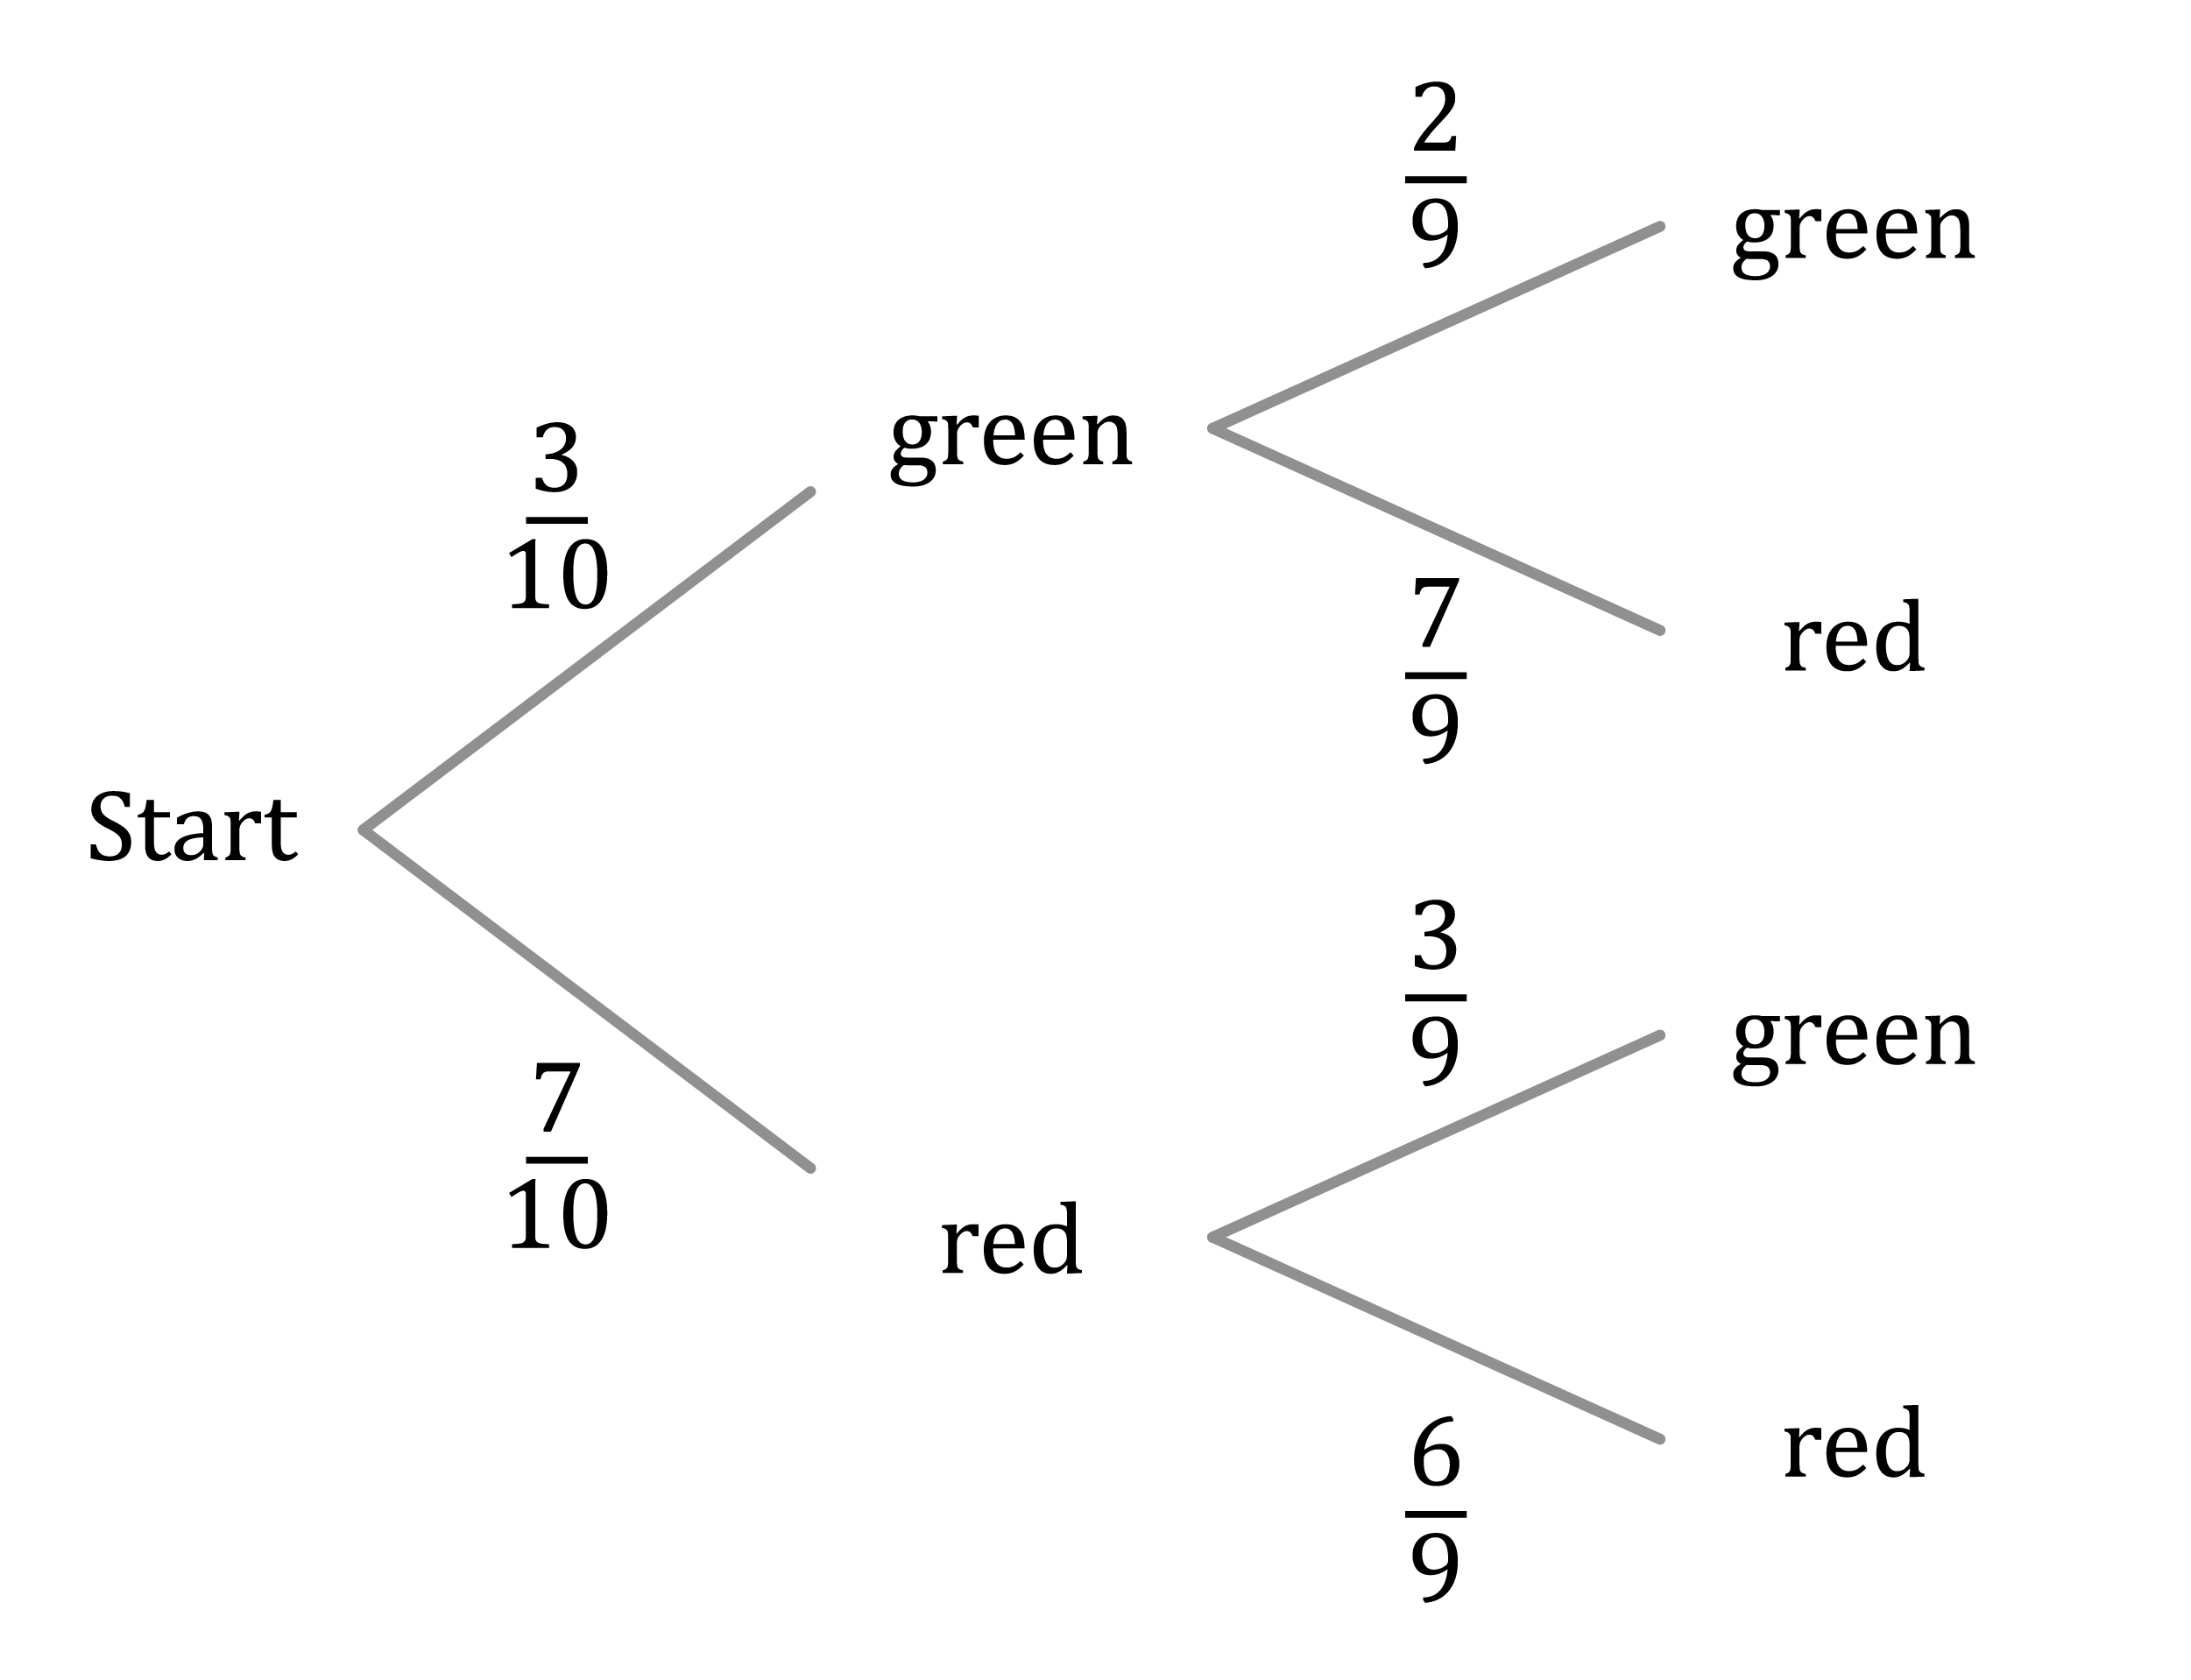
\includegraphics[scale=.06]{chance_tree}
\end{center}

\paragraph{Regola della catena} Per calcolare la probabilità di una qualsiasi foglia, che considero come una sequenza di esiti, bisogna individuare qual è il percorso che porta ad essa.
\begin{equation}
	P(\text{ramo}) = \text{prodotto delle probabilità dei sotto rami}
\end{equation}

\paragraph{Regola di fattorizzazione}
\begin{equation}
	P(\text{unione dei rami}) = \text{somma delle probabilità dei rami}
\end{equation}

\subsection{Indipendenza}
Vogliamo tradurre in linguaggio matematico il fatto che la probabilità di $B$ non cambia sapendo che accada $A$ e viceversa.
\begin{definition}
	Dati $n$ eventi $A_1, \ldots, A_n$, questi sono indipendenti se per ogni $k$ con $2 \leq k \leq n$ e per ogni scelta di interi $1 \leq i_1 < i_2< \ldots < i_k \leq n$ vale
	\begin{equation}
		\mathbb{P}(A_{i_1} \cap \ldots \cap A_{i_k}) = \mathbb{P}(A_{i_1}) \cdot  \ldots \cdot \mathbb{P}(A_{i_k})
	\end{equation}
\end{definition}

\begin{observation}
	Questa definizione equivale a dire che $P(A\vert B) = P(A)$ e $P(B \vert A) = P(B)$.
\end{observation}

\begin{observation}
	Se $P(A)=0$  oppure $P(A)=1$ allora $A$ è indipendente da qualsiasi altro evento.
\end{observation}

\begin{observation}
	Due eventi disgiunti non possono essere indipendenti a meno che uno dei due non sia trascurabile.
\end{observation}

\begin{observation}
	Due eventi possono essere indipendenti anche in presenza di una relazione causale. Viceversa due eventi possono essere dipendenti anche in assenza di una relazione causale.
\end{observation}

\subsubsection{Schema di Bernoulli}
Consideriamo $n$ prove ripetute di un esperimento in cui gli esiti sono successo, denominato come $1$ o insuccesso come $0$. Sia $p$ la probabilità di successo nella singola prova.
\begin{equation*}
	\Omega = \{(a_1, \ldots, a_n) \vert a_i \in \{0,1\}\} = \{0,1\}^n
\end{equation*}
Allora, visto che gli eventi sono indipendenti, la probabilità di una certa "stringa" (e.g. $(0,1,0)$) è:
\begin{align*}
	P(a_1, \ldots, a_n) & = P(a_1\text{ al 1° posto }) \cdot P(a_2\text{ al 2° posto }) \cdot \ldots \cdot P(a_n\text{ al n° posto }) \\
	& = p^{\#\text{ successi }} \cdot (1-p) ^ {\#\text{ insuccessi }} \\
	& = p^{\sum_{i=1}^{n}a_i} \cdot (1-p)^{n - \sum_{i=1}^{n}a_i} 
\end{align*}
% !TeX spellcheck = it_IT
\newpage
\section{Variabili aleatorie}
Le variabili aleatorie sono funzioni dello spazio di probabilità. Permettono di scrivere osservazioni diverse fatte su uno stesso spazio $\Omega$.
\begin{definition}[Variabile aleatoria]
	Dato un esperimento aleatorio, una variabile aleatoria è una funzione $X$ che associa ad ogni possibile risultato dell'esperimento un numero reale.
	\begin{equation}
		X : \Omega \to \mathbb{R}
	\end{equation}
	definita su uno spazio di probabilità.
\end{definition}

\begin{definition}[Legge di una variabile aleatoria]
	Sia $X: \Omega \to \mathbb{R}$ una variabile aleatoria, definiamo la sua legge o distribuzione di probabilità la funzione $P_X : \mathcal{P}(\mathbb{R}) \to \mathbb{R}$ data da:
	\begin{equation*}
		P_X(A) = P(X \in A) \qquad \forall A \subseteq \mathbb{R}
	\end{equation*}
	dove
	\begin{equation*}
		\{X\in A\} = X^{-1}(A) = \{\omega \in \Omega \vert X(\omega) \in A\}
	\end{equation*}
\end{definition}

\begin{proposition}
	$X^{-1}$ commuta con le operazioni insiemistiche e $P_X$ è una probabilità su $\mathbb{R}$.
\end{proposition}

\begin{definition}[Equidistribuzione]
	Due variabili aleatorie $X$ e $Y$ si dicono equidistribuite se hanno la stessa legge di probabilità.
	\begin{equation}
		P_X = P_Y
	\end{equation}
\end{definition}

\subsection{Discrete}
\begin{definition}[Variabile aleatoria discreta]
	Una variabile aleatoria $X$ si dice discreta se assume un numero finito o numerabile di valori (modalità) $a_1, \ldots, a_n, \ldots$.
\end{definition}

\begin{definition}[Funzione di massa]
	Data una v.a. discreta $X: \Omega \mapsto \{a_1, \ldots, a_n, \ldots\} \in \mathbb{R}$ definiamo la funzione di massa o densità discreta di $X$ la funzione
	\begin{equation*}
		P_X: \{a_1, \ldots, a_n, \ldots\} \mapsto \mathbb{R}
	\end{equation*}
	definita come
	\begin{equation}
		P_X(a_i) = P(X=a_i) = P_X\{a_i\}=P(X^{-1}(a_i))
	\end{equation}
	Ovvero associo ad ogni valore la probabilità della controimmagine di quel valore.\\\\
	Possiamo poi estendere $P_X$, per il XXXX definita solo nell'insieme discreto dei valori di $X$ (ovvero l'immagine di $\mathbb{R}$) e tutto $\mathbb{R}$ (ottenendo $p_X: \mathbb{R} \to \mathbb{R}$, ponendo:
	\begin{equation}
		p_X(a)=0 \qquad \forall a \notin \{a_1, \ldots\}
	\end{equation}
\end{definition}

\begin{note}
	La distribuzione di una v.a. discreta si rappresenta bene tramite un diagramma a barre.
\end{note}

Per eseguire il calcolo della probabilità relativa ad $X_i$ usando $P_X$:
\begin{align*}
	P(X=A) & = P(X^{-1}(A)) \\
	& = P(x=a_1 \cup x=a_2 \cup \ldots \cup x=a_i) \\
	& = \sum_{q_i \in A}P(X=a_i) \\
	& = \sum_{q_in \in A} p_X(a_i)
\end{align*}

\begin{example}
	Qual è la probabilità di avere almeno una testa in due lanci di dadi?
	\begin{equation*}
		A=\{1,2\} \Longrightarrow P(X\in\{1,2\}) = P(X=1) \cup P(X=2) = \frac{1}{4} + \frac{1}{2} = \frac{3}{4}
	\end{equation*}
\end{example}

\begin{example}
	Qual è la probabilità di avere almeno due teste in quattro lanci di dadi?\\
	Consideriamo lo spazio campionario $\Omega = \{0,1\}^4$ ($0$ croce e $1$ testa) e la variabile aleatoria $X$ che rappresenta il numero di teste.
	\begin{equation*}
		\Omega = \{(\omega_1, \omega_2, \omega_3, \omega_4) \vert w_j \in \{0,1\}\}
	\end{equation*}
	Abbiamo quindi:
	\begin{align*}
		P_X(0) & =\frac{1}{2} \cdot \frac{1}{2} \cdot \frac{1}{2} \cdot \frac{1}{2} = \frac{1}{16} \\
		P_X(1) & = \frac{1}{16} + \frac{1}{16} + \frac{1}{16} + \frac{1}{16} = \frac{4}{16} = \frac{1}{4} \\
		P_X(2) & = \frac{6}{16} = \frac{3}{8} \\
		P_X(3) & = \frac{1}{4} \\
		P_X(4) & = \frac{1}{16}
	\end{align*}
	La soluzione è:
	\begin{equation*}
		P(\geq 2 \text{ teste in 4 lanci }) = P_X(2) + P_X(3) + P_X(4) = \frac{3}{8} + \frac{1}{4} + \frac{1}{16} = 1 - \bigg(\frac{1}{16} + \frac{1}{4}\bigg)
	\end{equation*}
\end{example}

\begin{observation}
	La v.a. discreta $X$ può avere un insieme di valori finito o infinito. Nel primo caso allora $p(X\in A)$ è una somma finita $\forall A$. Altrimenti, se è numerabile, dobbiamo fare una serie:
	\begin{equation}
		\sum_{i=1}^{\infty} p(a_i) = \lim_{N \to \infty} \sum_{i=1}^{N}p(a_i)
	\end{equation}
\end{observation}

\begin{proposition}[Proprietà]
	Sia $X$ una v.a. discreta con funzione di massa $p_x$, allora valgono:
	\begin{itemize}
		\item $p_x(a_i) \geq 0 \qquad \forall i$
		\item $\sum_{i}p_x(a_i) = 1$
	\end{itemize}
	Se $q: \{a_1, a_2, \ldots\} \to \mathbb{R}$ è una funzione che soddisfa le proprietà allora esiste una variabile aleatoria $X$ di cui $q$ è la funzione di massa, ovvero $q=p_X$ per qualche $X$ v.a. discreta.
\end{proposition}
\begin{demostration}
	Vediamo le dimostrazioni delle due proprietà:
	\begin{itemize}
		\item $p_X(a_i) = P(X=a_i) = P(X^{-1}(a_i)) \geq 0$
		\item $\sum_{i}p_X(a_i) = \sum_i P(X=a_i) = P(\bigcup X^{-1}(a_i)) = P(\Omega) = 1$
	\end{itemize}
\end{demostration}

\subsection{Continue}
\begin{definition}[Variabile aleatoria continua]
	Sia $X$ una variabile casuale che assume tutti i valori di un intervallo (limitato o illimitato). Diciamo che essa è assolutamente continua con \textbf{densità} se$f$ se ad $X$ è associata una funzione $f:\mathbb{R} \mapsto \mathbb{R}$ tale che
	\begin{equation}
		\mathbb{P}\{X \in A\}=\mathbb{P}(a \leq X \leq b) = \int_{a}^{b} f(x) dx
	\end{equation}
\end{definition}

\begin{proposition}[Proprietà]
	Sia $X$ una v.a. continua con funzione di densità $f$ allora valgono:
	\begin{itemize}
		\item $f(x)\geq 0 \qquad \forall x$
		\item La misura dell'area sotto a grafico di tutta $f$ è $1$
	\end{itemize}
\end{proposition}

\subsection{Funzione di ripartizione}
Per studiare una legge di probabilità di una variabile aleatoria è conveniente usare una funzione su $\mathbb{R}$.
\begin{definition}[Funzione di ripartizione]
	La funzione di ripartizione su $X$ è
	\begin{equation}
		F_X:\mathbb{R}\to[0,1] \quad\quad F_X(x) = \mathbb{P}\{X \leq x\} = P_X((-\infty,x]) \qquad \forall x \in \mathbb{R}
	\end{equation}
	In pratica associa ad ogni $x \in \mathbb{R}$ la probabilità che $X$ assuma un valore al massimo pari ad $x$.
\end{definition}

\begin{proposition}
	Data $F=F_X$ la funzione di ripartizione di una variabile aleatoria $X$, valgono:
	\begin{itemize}
		\item $F$ è \textbf{non decrescente}
		\begin{equation}
			x < y \Longrightarrow F(X) \leq F(y)
		\end{equation}
		\item $\lim_{x \to -\infty}=0$, $\lim_{x \to + \infty}F(x) = 1$
		\item $F$ è \textbf{continua} a destra
		\begin{equation}
			\forall x \in \mathbb{R} \quad F(x_n) \to F(x)
		\end{equation}
		per ogni successione $x_n \to x \quad\quad x_n \geq x$
	\end{itemize}
\end{proposition}

\begin{proposition}
	La probabilità che $X$ cada in un dato intervallo $[a,b]$ per $a<b$ è
	\begin{equation}
		\mathbb{P}\{a < X \leq b\}=F(b)-F(a)
	\end{equation}
\end{proposition}

\subsubsection{Funzioni di variabili discrete}
Data una variabile aleatoria discreta $X$, la sua c.d.f. che assume valori $x_1, x_2, \ldots$ è
\begin{equation}
	F_X(t) = \sum_{x_i \leq t}p(x_i)
\end{equation}
Questa è una funzione a \textbf{gradini} che esegue un salto in ogni punto $x$ tale che $\mathbb{P}(X=x)>0$ di ampiezza pari alla probabilità di quel punto. Vale quindi
\begin{equation}
	\mathbb{P}\{X=x\} = F(x) - F_\_(x)
\end{equation}
\subsubsection{Funzioni di variabili continue}
Quando la variabile ha densità $f$ la sua funzione di ripartizione (\textbf{continua}) è
\begin{equation}
	F(x)=\int_{-\infty}^{x}dt
\end{equation}
o nel caso in cui è \textbf{continua a tratti} si ottiene:
\begin{equation}
	f(x) = \frac{dF(x)}{dx}
\end{equation}

\subsubsection{$\beta$-quantile}
\begin{definition}[$\beta$-quantile]
	Data una variabile aleatoria $X$ ed un numero $0 < \beta < 1$ il $\beta$-quantile è un numero $r_\beta$ tale che:
	\begin{equation}
		P\{X \leq r_\beta\} \geq \beta \qquad\qquad P\{X \geq r_\beta\} \geq 1-\beta
	\end{equation}
\end{definition}

\begin{observation}
	Se $F_X$ è invertibile, allora $\forall \beta \in (0,1)$ esiste unico il beta quantile e $r_\beta = F_X^{-1}(\beta)$.
\end{observation}

\subsection{Variabili discrete notevoli}
\subsubsection{Binomiali}
\begin{equation}
	B(n,p)
\end{equation}
Date $n$ prove ripetute di un esperimento con \textbf{due esiti}, chiamiamo uno di questi \textit{successo} con probabilità $0 < p < 1$. Sia $X$ la variabile che conta il numero di successi ($0, 1, \ldots,n$). Vale:
\begin{equation}
	\mathbb{P}(X=h)=\binom{n}{h}p^h(1-p)^{n-h} \quad\quad 0 \leq h \leq n
\end{equation}
Ovvero dati $h$ successi e $n-h$ insuccessi, calcoliamo il numero di modi di disporre i successi.

\begin{observation}
	Date due successioni $x_1,x_2, \ldots \in \mathbb{R}$ e $p_1, p_2, \ldots \in [0, \infty)$ tale che $\sum_{i=1}^{\infty}p_1 = 1$, possiamo definire una variabile discreta tramite
	\begin{equation}
		\Omega = \mathbb{N} \quad\quad \mathbb{P}(\{k\})=p_k \quad\quad X(k) = x_k
	\end{equation}
	ovvero dove
	\begin{equation*}
		\mathbb{P}_X(k) = \mathbb{P}(X = x_k) = p_k
	\end{equation*}
\end{observation}
Un caso particolare delle variabili binomiali è quando $n=1$, ovvero le variabili di \textbf{Bernoulli}.

\subsubsection{Geometriche}
\begin{equation}
	G(p)
\end{equation}
Consideriamo la stessa situazione delle variabili binomiali ma definiamo $X$ come l'istante del primo successo, ovvero il numero $h$ tale che alla prova $h$-esima si verifichi il primo successo. Vale:
\begin{equation}
	P(X=h)=(1-p)^{h-1}p \quad\quad h \in \mathbb{N}_0
\end{equation}
Questo corrisponde a dire, dato l'evento $A_i$ successo della prova $i$-esima,
\begin{equation*}
	\mathbb{P}(X=h) = \mathbb{P}(A^c_1 \cap A^c_2 \cap \ldots \cap A^c_{h-1} \cap A_h) = \mathbb{P}(A^c_1) \cdot \mathbb{P}(A^c_2) \cdot \ldots \cdot \mathbb{P}(A^c_{h-1}) \cdot \mathbb{P}(A_h) = (1-p)^{h-1}p
\end{equation*} 

\begin{observation}[Assenza di memoria]
	Le variabili geometriche hanno assenza di memoria, ovvero
	\begin{equation}
		\mathbb{P}\{X=n+h \vert X >n \} = \mathbb{P}\{X=h\}
	\end{equation}
\end{observation}

\subsubsection{Ipergeometriche}
\begin{equation}
	I(n,h,r)
\end{equation}
Prendiamo ad esempio un'urna con $n$ biglie di cui $0 \leq h \leq n$ sono bianche e $n-h$ nere. Estraiamo $r \leq n$ biglie senza reinserirle. La variabile che conta quante biglie estratte $k$ sono bianche ha funzione di massa
\begin{equation}
	\mathbb{P}(X=k) = \frac{\binom{h}{k}\binom{n-h}{r-k}}{\binom{n}{r}} \quad\quad k=0,\ldots, h
\end{equation}
\begin{proposition}[Identità di Vandermonde]
	Date $k$ biglie bianche e $r-k$ nere, il numero di scelte possibili è
	\begin{equation*}
		\binom{h}{k}\binom{n-h}{r-k}
	\end{equation*}
	mentre il numero totale di scelte è 
	\begin{equation*}
		\binom{n}{r}
	\end{equation*}
	Otteniamo quindi
	\begin{equation}
		\sum_{k=0}^{h} \binom{h}{k}\binom{n-h}{r-k} = \binom{n}{r}
	\end{equation}
	che mostra anche $\sum_{k=0}^{h}\mathbb{P}(X=k) = 1$
\end{proposition}

\subsubsection{Poisson}
\begin{equation}
	P(\lambda)
\end{equation}
Una variabile è di Poisson quando
\begin{equation}
	\mathbb{P}(X=h)=e^{-\lambda}\frac{\lambda^h}{h!} \quad\quad h \in \mathbb{N}, \lambda>0
\end{equation}
Dato che è una buona approssimazione di una distribuzione binomiale quando $n$ è grande, $p$ è piccolo $np$ è circa $\lambda$, possiamo dire che conta il numero di successi quando il numero di prove è alto e la probabilità è bassa. Viene anche detta degli \textbf{eventi rari} (eruzioni vulcaniche, particelle $\alpha$ emesse da una sorgente radioattiva).

\subsection{Variabili con densità notevoli}
Consideriamo i casi in cui esiste una funzione di densità non negativa di integrale unitario su tutto $\mathbb{R}$ $f_X$ tale che
\begin{equation}
	\mathbb{P}(X \in [a,b]) = \mathbb{P}(X \in (a,b)) = \int_{a}^{b} f_X(t)dt
\end{equation}

\subsubsection{Uniformi su intervalli}
Dati due numeri reali $a < b$, la densità uniforme sull'intervallo $[a,b]$ è
\begin{equation}
	f(t) = \begin{cases}
		\frac{1}{b-a} & a < t < b\\
		0 & \text{altrove}
	\end{cases}
\end{equation}
La c.d.f. è
\begin{equation}
	F(t)=\begin{cases}
		0 & t \leq a \\
		\frac{t}{b-a} & 0 < t \leq b \\
		1 & t>b
	\end{cases}
\end{equation}
Ad esempio un numero preso a caso tra $0$ e $1$.

\subsubsection{Esponenziali}
Dato il parametro $\lambda>0$ la densità è
\begin{equation}
	f(x)=\begin{cases}
		\lambda e^{-\lambda t} & t >0 \\
		0 & t \leq 0
	\end{cases}
\end{equation}
La c.d.f. è
\begin{equation}
	F(t) = \begin{cases}
		1-e^{-\lambda t} & t>0\\
		0 & t \leq 0
	\end{cases}
\end{equation}
Descrive ad esempio il tempo di attesa tra due eventi aleatori, come tra le chiamate di un call center.
\begin{observation}
	Questa variabile prende solo valori positivi
	\begin{equation*}
		\mathbb{P}\{X \leq 0\}= 0
	\end{equation*}
\end{observation}

\subsubsection{Gamma}
\begin{equation}
	\Gamma(r, \lambda)
\end{equation}
\begin{definition}[Gamma di Eulero]
	Rappresenta l'estensione del fattoriale ai numeri non interi.
	\begin{equation}
		\Gamma(r) = \int_{0}^{+\infty} x^{r-1}e^{-x}dx \quad\quad r>0
	\end{equation}
	Valgono
	\begin{equation*}
		\Gamma(1) = 1 \quad\quad \Gamma(r) = (r-1)\Gamma(r-1)
	\end{equation*}
\end{definition}

\begin{definition}
	La densità Gamma di parametri $r, \lambda > 0$ è
	\begin{equation}
		f(x) = \begin{cases}
			\frac{1}{\Gamma(r)}\lambda^r x^{r-1}e^{-\lambda x} & x >0\\
			0 & x \leq 0
		\end{cases}
	\end{equation}
\end{definition}

\begin{proposition}
	Date due variabili \textbf{indipendenti} $X$ e $Y$ con densità $\Gamma(r, \lambda)$ e $\Gamma(s, \lambda)$ allora $X+Y$ ha densità $\Gamma(r+s, \lambda)$.
\end{proposition}

\begin{observation}[Parametri]
	Il parametro $r$ rappresenta la forma e $\lambda$ il tasso di decadimento. In alcuni casi invece di $\lambda$ viene usato $s=\frac{1}{\lambda}$, ovvero il fattore di scala. In quel caso la densità diventa
	\begin{equation*}
		f(x) = \begin{cases}
			\frac{1}{\Gamma(r)} \frac{1}{s} \bigg(\frac{x}{s}\bigg)^{r-1} e^{-\frac{x}{s}} & x >0\\
			0 & x \leq 0
		\end{cases}
	\end{equation*}
\end{observation}

\begin{observation}
	La densità \textbf{esponenziale} di parametro $\lambda$ corrisponde a $\Gamma(1, \lambda)$.
\end{observation}

\begin{proposition}
	Una variabile $X$ con densità Gamma ha tutti i momenti e vale
	\begin{equation}
		\mathbb{E}[X^\beta]=\frac{\Gamma(r + \beta)}{\Gamma(r)\lambda^\beta} \quad\quad \forall \beta > 0
	\end{equation}
\end{proposition}

\subsubsection{Pareto}
Dati $x_m, \alpha > 0$ la densità è
\begin{equation}
	f(t) = \begin{cases}
		\alpha x_m^\alpha t^{-1-\alpha} & t> x_m \\
		0 & t \leq x_m
	\end{cases}
\end{equation}
La densità è non nulla dopo la soglia $x_m$ e al diminuire di $\alpha$ ha una coda sempre più pesante. La c.d.f. è
\begin{equation}
	F(t) = \begin{cases}
		1 & t < x_m \\
		1-(\frac{x_m}{t})^\alpha & t \geq x_m
	\end{cases}
\end{equation}
Chiamata anche \textbf{power law}, serve a descrivere fenomeni in cui eventi estremi hanno una buona probabilità di avvenire, come la distribuzione della ricchezza nella società.

\subsubsection{Gaussiane standard}
Viene indicata con $N(0,1)$ e ha densità
\begin{equation}
	\varphi(x) = \frac{1}{\sqrt{2\pi}}e^{\frac{-x^2}{2}}
\end{equation}
e c.d.f.
\begin{equation}
	\Phi(x)=\frac{1}{\sqrt{2\pi}}\int_{-\infty}^{x}e^{\frac{-t^2}{2}}dt
\end{equation}

\begin{observation}
	Questa densità è una funzione pari ($\varphi(x) = \varphi(-x)$). Di conseguenza, dati $x \in \mathbb{R}$ e $0 < \alpha < 1$, si ha
	\begin{equation}
		\Phi(-x) = 1 - \Phi(x) \quad\quad q_{1-\alpha} = -q_\alpha
	\end{equation}
	Di conseguenza, se $X$ è una variabile aleatoria $N(0,1)$, valgono
	\begin{equation}
		\mathbb{P}\{-t \leq X \leq t\} = \Phi(t) - \Phi(-t) = 1\Phi(t) -1
	\end{equation}
	\begin{equation}
		\Phi(0) = \mathbb{P}\{X \geq 0\} = \mathbb{P}\{X \leq 0\} = \frac{1}{2}
	\end{equation}
\end{observation}

\subsubsection{Chi-Quadro}
\begin{definition}[Densità Chi-Quadro]
	Se $X_1, \ldots, X_n$ sono variabili Gaussiane Standard indipendenti, la variabile $(X_1^2 + \ldots + X_n^2)$ ha densità $\Gamma(\frac{n}{2}, \frac{1}{2})$, ovvero Chi-Quadro $\mathcal{X}^2(n)$ con $n$ gradi di libertà.
\end{definition}

\begin{proposition}[Approssimazioni]
	Definiamo una variabile $C_n = X_1^2 + \ldots + X_n^2$ con $X_i$ Gaussiane standard indipendenti. Per $n\to \infty$ (in generale $n \geq 80$) valgono:
	\begin{itemize}
		\item Per la LGN $C_n \to 1$, quindi $\frac{C_n}{n} \approx 1$
		\item Per il TCL $\frac{C_n -n}{\sqrt{2n}}$ converge alla variabile Gaussiana Standard
	\end{itemize}
\end{proposition}
\subsubsection{Student}
\begin{definition}
	Date due variabili $X$ e $C_n$ con densità $N(0,1)$ e $\mathcal{X}^2(n)$, definiamo la densità di Student come
	\begin{equation}
		T_n = \frac{X}{\sqrt{\frac{C_n}{n}}} = \sqrt{n} \frac{X}{\sqrt{C_n}}
	\end{equation}
	con densità
	\begin{equation}
		f_{T_n}(t) = \frac{\Gamma(\frac{n}{2}+\frac{1}{2})}{\sqrt{n\pi}\Gamma(\frac{n}{2})}\bigg(1+\frac{t^2}{n}\bigg)^{-\frac{n}{2}-\frac{1}{2}}
	\end{equation}
\end{definition}

\begin{proposition}
	La densità di Student è una funzione pari, di conseguenza valgono
	\begin{equation}
		F_n(-x)=1-F_n(x) \quad\quad\quad \tau_{(\alpha, n)} = -\tau_{(1-\alpha, n)}
	\end{equation}
\end{proposition}

\begin{theorem}
	Consideriamo la successione $(T_n)_{n\geq 1}$ di variabili di Student. Questa converge in distribuzione alla variabile $N(0,1)$. Può quindi essere usata per sostituire una Gaussiana, prestando attenzione al fatto che però tende a $0$ più lentamente per $\lvert x \rvert \to \infty$ (\textbf{code pesanti}).
\end{theorem}

\subsubsection{Gaussiane non standard}
\begin{equation}
	N(m, \sigma^2)
\end{equation}
Data $X$ una variabile Gaussiana Standard, dati $\sigma >0$ e $m \in \mathbb{R}$, consideriamo la variabile aleatoria $Y = \sigma X +m$. La sua densità è
\begin{equation}
	f_Y(t) = \frac{1}{\sigma}f_X\bigg(\frac{t-m}{\sigma}\bigg) = \frac{1}{\sqrt{2 \pi}\sigma}e^{-\frac{(t-m)^2}{2\sigma^2}}
\end{equation}
mentre la sua c.d.f. è
\begin{equation}
	F_Y(t)= \mathbb{P}\{Y \leq t\} = \mathbb{P}\{\sigma X + m \leq t\} = \mathbb{P}\bigg(X \leq \frac{t-m}{\sigma}\bigg) = \Phi \bigg(\frac{t-m}{\sigma}\bigg)
\end{equation}

\begin{theorem}[Teorema di Cochran]
	Siano $X_1, \ldots, X_n$ variabili Gaussiane i.i.d. $N(m, \sigma^2)$. Valgono:
	\begin{itemize}
		\item $\bar{X}_n$ e $S_n^2$ sono \textbf{indipendenti}
		\item $\bar{X}$ ha densità $N(m, \frac{\sigma^2}{n})$
		\item $\frac{n-1}{\sigma^2}S_n^2$ ha densità $\mathcal{X}^2(n-1)$
		\item $T=\sqrt{n}\frac{(\bar{X}_n - m)}{S}$ ha densità $T(n-1)$
	\end{itemize}
\end{theorem}

\subsubsection{Cambio di variabile}
Data la variabile aleatoria $X: \Omega \to \mathbb{R}$ con densità $f$ e una funzione $h: \mathbb{R} \to \mathbb{R}$, vogliamo la densità della variabile aleatoria composta 
\begin{equation*}
	Y: \Omega \to \mathbb{R} \quad\quad Y=h \circ X
\end{equation*}
Se è possibile calcolare la c.d.f. di $Y$
\begin{equation*}
	F_Y(y)=\mathbb{P}\{Y \leq y\} = \mathbb{P}\{h(X) \leq y\}
\end{equation*}
ed è \textbf{continua} e differenziabile, allora è sufficiente derivarla per ottenere la densità di $Y$.
\begin{proposition}[Cambio di variabile]
	Data $X$ una variabile aleatoria con densità $f_X$, supportata su un intervallo aperto $A$ ($f_X$ nulla su $A^c$). Data una funzione $h: A \to B$, con $B$ un intervallo aperto, \textbf{biunivoca}, \textbf{differenziabile} e con \textbf{inversa differenziabile}. Allora $Y = h \circ X$ ha densità
	\begin{equation}
		f_Y(y)=\begin{cases}
			f_X(h^{-1}(y)) \cdot \bigg\lvert \frac{dh^{-1}(y)}{dy}\bigg\rvert & y \in B\\
			0 & y \notin B
		\end{cases}
	\end{equation}
\end{proposition}

\subsection{Valore atteso}
Applichiamo il concetto di \textit{media campionaria} e di \textit{varianza campionaria} anche alle variabili aleatorie.
\begin{definition}[Valore atteso]
	Data una variabile discreta $X$ con funzione di massa $p_X$, si dice che questa ha valore atteso se
	\begin{equation*}
		\sum_{i}\lvert x_i \rvert p_X(x_i) < +\infty
	\end{equation*}
	e vale
	\begin{equation}
		\mathbb{E}[X]=\sum_{i}x_ip_X(x_i)
	\end{equation}
	Se $X$ è con densità e
	\begin{equation*}
		\int_{-\infty}^{+\infty} \lvert x \rvert f_X(x) dx < + \infty
	\end{equation*}
	allora il valore atteso è
	\begin{equation}
		\mathbb{E}[X]=\int_{-\infty}^{+\infty}t f_X(t)dt
	\end{equation}
\end{definition}

\begin{note}
	Il valore atteso è anche chiamato \textbf{momento primo} o speranza matematica.
\end{note}

\begin{observation}
	Dato che il valore atteso dipende solo dalla funzione di massa o dalla densità, ovvero solo dalla legge $\mathbb{P}_X$ di $X$, allora se due variabili sono \textbf{equi distribuite} hanno anche lo stesso valore atteso.
\end{observation}

\begin{observation}
	Se $X$ prende solo valori positivi, possiamo ammettere che $E[X]$ possa assumere il valore $+\infty$.\\
	Nel caso discreto vuol dire che $x_1, x_2, \ldots$ sono sempre positivi e quindi ha senso
	\begin{equation*}
		\mathbb{E}[X]=\sum_{i=1}^{+\infty} x_i p(x_i)
	\end{equation*}
	Nel caso con densità significa che $f(x)=0 \quad x<o$ e quindi ha senso
	\begin{equation*}
		\mathbb{E}[X] = \int_{0}^{+\infty} xf(x)dx \in [0, +\infty]
	\end{equation*}
	In generale
	\begin{equation}
		\mathbb{E}[\lvert X \rvert] < + \infty
	\end{equation}
\end{observation}

\begin{proposition}
	Valgono le seguenti proprietà:
	\begin{itemize}
		\item \textbf{Linearità}:
		\begin{itemize}
			\item $\mathbb{E}[X+Y]=\mathbb{E}[X]+\mathbb{E}[Y]$
			\item $\mathbb{E}[aX+b]=a\mathbb{E}[X] + b$, in particolare $\mathbb{E}[b] = b$
		\end{itemize}
		\item \textbf{Monotonia}: se $X \geq 0$ allora $\mathbb{E}[X] \geq 0$ e se $X \geq Y$ allora $\mathbb{E}[X] \geq \mathbb{E}[Y]$. In particolare $\lvert \mathbb{E}[X]\rvert \leq \lvert \mathbb{E}[\lvert X \rvert]$
	\end{itemize}
\end{proposition}

\subsubsection{Valore atteso di trasformazioni}
Supponiamo di voler calcolare il valore atteso di trasformazioni di una variabile aleatoria $X$, ovvero $Y=g(x) \quad g:\mathbb{R} \to \mathbb{R}$.
\begin{proposition}[Valore atteso di trasformazioni discrete]
	Se $X$ è discreta e
	\begin{equation*}
		\sum_{i} \lvert g(x_i) \rvert p(x_i) < +\infty
	\end{equation*}
	allora
	\begin{equation}
		\mathbb{E}[g(X)] = \sum_{i} g(x_i)p(x_i)
	\end{equation}
\end{proposition}
\begin{proposition}[Valore atteso di trasformazioni con densità]
	Se $X$ è con densità e
	\begin{equation*}
		\int_{-\infty}^{+\infty}\lvert g(x)\rvert f(x)dx < +\infty
	\end{equation*}
	allora
	\begin{equation}
		\mathbb{E}[g(X)] = \int_{-\infty}^{+\infty} g(x) f(x)dx
	\end{equation}
\end{proposition}
	
\subsubsection{Momenti}
\begin{definition}[Momento]
	Data $X$ una variabile aleatoria, chiamiamo momento di ordine $n$ di $X$ il valore atteso di $X^n$
	\begin{equation}
		\mathbb{E}[X^n]
	\end{equation}
\end{definition}

\begin{observation}
	Se una variabile discreta assume solo valori finiti, tutti i momenti sono finiti. Se una variabile con densità è diversa da $0$ solo su un intervallo limitato, tutti i momenti sono finiti.
\end{observation}

\begin{proposition}[Disuguaglianza di Markov]
	Se $X$ è una variabile aleatoria a valori positivi e $a>0$ vale
	\begin{equation}
		\mathbb{P}\{X \geq a\} \leq \frac{1}{a}\mathbb{E}[X]
	\end{equation}
\end{proposition}

\subsubsection{Varianza di una variabile aleatoria}
\begin{definition} [Varianza]
	Se $X$ ammette momento secondo, la sua varianza è
	\begin{equation}
		Var(X) = \mathbb{E}[(X-\mathbb{E}[X])^2] = \mathbb{E}[X^2]-\mathbb{E}[X]^2
	\end{equation}
	e lo \textbf{scarto quadratico medio} o \textbf{deviazione standard} è
	\begin{equation}
		\sigma(X) = \sqrt{Var(X)}
	\end{equation}
\end{definition}

\begin{proposition}[Disuguaglianza di Chebyshev]
	Data $X$ una variabile aleatoria e $d>0$, vale
	\begin{equation}
		\mathbb{P}\{\lvert X - \mathbb{E}\rvert > d\} \leq \frac{Var(X)}{d^2}
	\end{equation}
	Ovvero la probabilità che $X$ si allontani dal suo valore atteso più di $d$ è minore o uguale di $\frac{Var(X)}{d^2}$.
\end{proposition}

\begin{observation}
	La varianza di una variabile $X$ vale $0$ solo se questa è costante tranne che per un insieme trascurabile
	\begin{equation*}
		\mathbb{P}\{\lvert X - \mathbb{E}[X] \rvert \neq 0\} = 0
	\end{equation*}
\end{observation}

\begin{proposition}[Scaling]
	La proprietà di scaling implica che vale:
	\begin{equation}
		Var(a X+b) = a^2 Var(X)
	\end{equation}
	e in particolare $Var(b)=0$.
\end{proposition}

\subsubsection{Momenti notevoli}
Vediamo i momenti delle variabili notevoli.
\paragraph{Variabili binomiali}
Per una variabile di Bernoulli, che può valere $0$ o $1$, vale
\begin{align}
	& \mathbb{E}[X^k] = 0 \cdot \mathbb{P}(X=0)+1\cdot \mathbb{P}(X=1) = 0 \cdot (1-p) + 1 \cdot p = p \\
	&\quad\quad Var(X)=p-p^2=p(1-p) \quad\quad k \geq 1
\end{align}
Dato che una variabile Binomiale può essere vista come somma di variabili di Bernoulli, vale
\begin{equation}
	\mathbb{E}[X] = np \quad\quad Var(X) = np(1-p)
\end{equation}

\paragraph{Variabili di Poisson}
Dato che assumono solo valori positivi:
\begin{equation}
	\mathbb{E}[X] = \sum_{h=0}^{+\infty}he^{-\lambda}\frac{\lambda^h}{h!} = \lambda e^{-\lambda}\sum_{h=1}^{+\infty}\frac{\lambda{h-1}}{(h-1)!} = \lambda e^{-\lambda}\sum_{k=0}^{+\infty}\frac{\lambda^k}{k!}=\lambda
\end{equation}
\begin{equation}
	\mathbb{E}[X^2]=\lambda + \lambda^2 \quad\quad Var(X)=\lambda
\end{equation}

\paragraph{Variabili uniformi su intervalli finiti}
Data una variabile $X$ con densità uniforme su $[a,b]$, vale:
\begin{equation}
	\mathbb{E}[X] = \int_{a}^{b}\frac{x}{b-a}dx = \frac{x^2}{2(b-a)}\bigg\vert^b_a = \frac{b^2-a^2}{2(b-a)}=\frac{a+b}{2}
\end{equation}
\begin{equation}
	\mathbb{E}[X^2] = \int_{a}^{b}\frac{x^2}{b-a}dx = \frac{x^3}{3(b-a)}\bigg\vert^b_a = \frac{b^3-a^3}{3(b-a)}=\frac{a^2+ab+b^2}{3} \quad\quad Var(X) = \frac{(b-a)^2}{12}
\end{equation}

\paragraph{Variabili esponenziali}
Vale:
\begin{equation}
	\mathbb{E}[X] = \int_{0}^{+\infty}\land x e^{-\lambda x}dx=\frac{1}{\lambda}
\end{equation}
e più in generale
\begin{equation}
	\mathbb{E}[X^n]=\frac{n!}{\lambda^n}
\end{equation}
Quindi anche
\begin{equation}
	Var(X) = \frac{1}{\lambda^2}
\end{equation}

\paragraph{Densità Gamma}
Vale:
\begin{equation}
	\mathbb{P}\{a < Y < b\} = \mathbb{P}\bigg\{\frac{a-m}{\sigma} < X < \frac{b-m}{\sigma}\bigg\}
\end{equation}
E in particolare:
\begin{equation}
	\mathbb{E}[X] = \frac{r}{\lambda} \quad\quad \mathbb{E}[X^2] = \frac{(r+1)r}{\lambda^2} \quad\quad Var(X)=\frac{r}{\lambda^2}
\end{equation}

\paragraph{Variabili Gaussiane standard}
Se $X$ è Gaussiana Standard, notiamo che possiede tutti i momenti
\begin{equation}
	\frac{1}{\sqrt{2\pi}}\int_{-\infty}^{+\infty}\lvert x\rvert^ne^{-\frac{x^2}{2}} dx < +\infty
\end{equation}
I momenti dispari valgono:
\begin{equation}
	\mathbb{E}[X^{2h+1}] = \frac{1}{\sqrt{2\pi}}\int_{-\infty}^{+\infty}x^ne^{-\frac{x^2}{2}}dx = \lim_{M \to \infty}\frac{1}{\sqrt{2\pi}}\int_{-M}^{+M}x^ne^{-\frac{x^2}{2}}dx=0
\end{equation}
mentre quelli pari, guardando ad esempio il momento secondo
\begin{equation}
	\mathbb{E}[X^2]=\frac{1}{\sqrt{2\pi}}\int_{-\infty}^{+\infty}x^2e^{-\frac{x^2}{2}}dx = \frac{-xe^{-\frac{x^2}{2}}}{\sqrt{2\pi}}\bigg\vert^{+\infty}_{-\infty}+\frac{1}{\sqrt{2\pi}}\int_{-\infty}^{+\infty}e^{-\frac{x^2}{2}}dx = 1 \quad\quad Var(X)=1
\end{equation}
e più in generale
\begin{equation}
	\mathbb{E}[X^{2h+2}]=(2h+1)\mathbb{E}[X^{2h}]
\end{equation}

\paragraph{Variabili di Student}
Una variabile di Student ha momenti finiti fino all'ordine $(n-1)$ e quelli di ordine dispari quando esistono sono nulli.

\paragraph{Variabili Gaussiane}
Data $Y=\sigma X + m$, per linearità del valore atteso
\begin{equation}
	\mathbb{E}[Y] = \mathbb{E}[\sigma X + m] = m \quad\quad Var(Y)=Var(\sigma X +m)=\sigma^2Var(X) = \sigma^2
\end{equation}

\subsection{Variabili doppie}
Dato un esperimento casuale con spazio di probabilità $(\Omega, p)$, una variabile casuale doppia è il dato di una coppia $(X,Y)$ di variabili casuali che ad ogni $\omega \in \Omega$ associa una coppia $(x,y) \in \mathbb{R}^2$.
\begin{equation}
	(X,Y): \Omega \mapsto \mathbb{R}^2 \qquad \qquad \omega \mapsto(X(\omega),Y(\omega))
\end{equation}

\subsubsection{Distribuzione congiunta}
\begin{definition}[Distribuzione congiunta]
	Data una variabile doppia $(X,Y): \Omega \mapsto\mathbb{R}^2$ definiamo la sua legge congiunta come la funzione $P_{\{X,Y\}}: \mathbb{P}(\mathbb{R}^2)\mapsto\mathbb{R}$ data da:
	\begin{align*}
		P_{\{X,Y\}}(A)&  = P\{(X,Y) \in A\} \\
		&= P((X,Y)^{-1}(A)) \\
		& = P\{\omega \in \Omega \vert (X,Y)(\omega)\in A\}
	\end{align*} 
\end{definition}

\begin{definition}[Distribuzioni marginali]
	Data una variabile doppia $(X,Y)$ possiamo considerare separatamente le leggi delle due componenti $\mathbb{P}_X$ e $\mathbb{P}_Y$. Queste sono dette \textbf{leggi marginali}.\\
	Se $I \subseteq \mathbb{R}$, valgono
	\begin{equation}
		\mathbb{P}_X(I)=\mathbb{P}_{(X,Y)}(I \times \mathbb{R}) \quad\quad\quad \mathbb{P}_Y(I)=\mathbb{P}_{(X,Y)}(\mathbb{R}\times I)
	\end{equation}	
\end{definition}

\begin{note}
	La distribuzione \textbf{congiunta} porta informazioni non solo sulle leggi marginali ma anche sulla relazione tra $X$ e $Y$.
\end{note}

\subsubsection{Variabili doppie discrete}
Una variabile doppia $(X,Y)$ è discreta se la sua immagine è concentrata in un insieme finito o numerabile di punti $(x_i, y_j)$. La sua \textbf{distribuzione di probabilità} è
\begin{equation}
	p(x_i,y_j) = \mathbb{P}(X=x_i, Y=y_j)
\end{equation}
e se $A\subseteq \mathbb{R}^2$
\begin{align*}
	\mathbb{P}_{(X,Y)}(A) & = \mathbb{P}\{(X,Y) \in A\} \\
	& = \sum_{(x_i, y_j) \in A}p(x_i, y_j)
\end{align*}

\begin{observation}
	Osserviamo che:
	\begin{itemize}
		\item $p(x_i,y_j) \geq 0 \qquad \forall i,j$ e $\sum_{i}\sum_jp(x_i,y_j)=1$
		\item La funzione di massa congiunta determina le funzioni di massa marginali
		\item Le funzioni di massa marginali non determinano quella congiunta
	\end{itemize}
\end{observation}

\begin{proposition}
	Se una variabile doppia è discreta con funzione di massa, lo sono anche le sue componenti
	\begin{equation}
		p_X(x_i) = \sum_{j=1}^{+\infty} p(x_i,y_j) \quad\quad p_X(y_j) = \sum_{i=1}^{+\infty} p(x_i,y_j)
	\end{equation}
\end{proposition}
\subsubsection{Variabili doppie con densità}
Una variabile doppia $(X,Y)$ è con densità se esiste una funzione $f : \mathbb{R}^2 \to [0,\infty)$ integrabile e con $\int\int_{\mathbb{R}^2}f(x,y)dxdy=1$ tale che valga
\begin{equation}
	\mathbb{P}_{(X,Y)}(A) = \mathbb{P}\{(X,Y) \in A\} = \int\int_A f(x,y) dxdy \quad\quad A \subseteq \mathbb{R}^2
\end{equation}

\begin{theorem}[Teorema di Fubini-Tonelli]
	Dato un insieme rettangolare $A = A_1 \times A_2$ vale
	\begin{equation}
		\int\int_A f(x,y)dxdy = \int_{A_1} \bigg(\int_{A_2} f(x,y)dy\bigg)dx =  \int_{A_2} \bigg(\int_{A_1} f(x,y)dx\bigg)dy 
	\end{equation}
\end{theorem}

\begin{proposition}
	Se una variabile doppia ha densità, anche le sue componenti la hanno
	\begin{equation}
		f_X(x) = \int_{-\infty}^{+\infty}f(x,y)dy \quad\quad f_Y(y) = \int_{-\infty}^{+\infty}f(x,y)dx
	\end{equation}
\end{proposition}

\begin{observation}
	A differenza del caso discreto se $X$ e $Y$ sono con densità non è detto che anche $X,Y)$ la abbia. Ad esempio $(X,X)$.
\end{observation}

\subsection{Indipendenza di variabili aleatorie}
\begin{definition}[Variabili aleatorie indipendenti]
	Le variabili aleatorie $X_1, \ldots, X_n:\Omega \to \mathbb{R}$ si dicono indipendenti se, presi comunque $A_1, \ldots, A_n \subseteq \mathbb{R}$ vale
	\begin{equation}
		\mathbb{P}(X_1 \in A_1, \ldots, X_n \in A_n) = \mathbb{P}(X_1 \in A_1) \cdot \ldots \cdot \mathbb{P}(X_n \in A_n)
	\end{equation} 
\end{definition}

\subsubsection{Indipendenza di variabili doppie}
\begin{proposition}[Indipendenza di variabili doppie discrete]
	Date due variabili discrete $X$ e $Y$ con immagine nei punti $x_i$ e $y_j$, sono indipendenti se e solo se vale
	\begin{equation}
		p(x_i, y_j) = p_X(x_i) \cdot p_Y(y_j) \quad\quad \forall(x_i, y_j)
	\end{equation}
\end{proposition}

\begin{proposition}[Indipendenza di variabili doppie con densità]
	Date due variabili $X$ e $Y$ tale che $(X,Y)$ abbia densità, sono indipendenti se e solo se vale
	\begin{equation}
		f(x,y) = f_X(x) \cdot f_Y(y) \quad\quad \forall(x,y)
	\end{equation}
\end{proposition}

\begin{observation}
	Due variabili aleatorie doppie possono avere le stesse distribuzioni marginali ma essere diverse, ad esempio perché in un caso le componenti sono indipendenti e nell'altro no.
\end{observation}

\subsubsection{Indipendenza di funzioni di variabili indipendenti}
Funzioni di più variabili indipendenti sono indipendenti se la stessa variabile non compare in due funzioni diverse.

\begin{proposition}
	Se $X,Y:\Omega \to \mathbb{N}$ sono variabili discrete a valori naturali e indipendenti e sia $Z=X+Y$ si ha
	\begin{equation}
		p_Z(n) = \sum_{h=0}^{n}p_X(h) \cdot p_Y(n-h)
	\end{equation}
	In particolare se $X$ e $Y$ sono binomiali $B(n,p)$ e $B(m,p)$, allora $Z=X+Y$ è binomiale $B(n+m,p)$.
\end{proposition}
\begin{proposition}
	Se $X$ e $Y$ sono variabili con densità e indipendenti e sia $Z=X+Y$ si ha
	\begin{equation}
		f_Z(z)=\int_{-\infty}^{+\infty}f_X(x)f_Y(z-x)dx = \int_{-\infty}^{+\infty}f_Y(y)f_X(z-y)dy
	\end{equation}
	In particolare se $X$ e $Y$ sono Gaussiane $N(m_1,\sigma_1^2)$ e $N(m_2,\sigma_2^2)$, allora $Z=X+Y$ è Gaussiana $N(m_1+m_2, \sigma_1^2+\sigma_2^2)$.
\end{proposition}

\begin{proposition}
	Se $X$ e $Y$ sono variabili aleatorie indipendenti, allora per tutte le funzioni $h,k: \mathbb{R} \to \mathbb{R}$, anche $h(X)$ e $k(Y)$ lo sono.
\end{proposition}

\begin{proposition}
	Vediamo le proprietà di \textbf{riproducibilità}:
	\begin{itemize}
		\item Siano $X \sim B(m,p)$ e $Y \sim B(h,p)$ \underline{indipendenti}, allora $X+Y \sim B(m+h,p)$
		\item Siano $X \sim P(\lambda)$ e $Y \sim P(\mu)$ \underline{indipendenti}, allora $X+Y \sim P(\lambda+\mu)$
		\item Siano $X \sim N(m_1, \sigma_1^2)$ e $Y \sim N(m_2, \sigma_2^2)$ \underline{indipendenti}, allora $X+Y \sim N(m_1+m_2, \sigma_1^2+\sigma_2^2)$
	\end{itemize}
\end{proposition}

\subsection{Correlazione}
\begin{proposition}
	Date due variabili aleatorie $X$ e $Y$ con valore atteso, allora $X+Y$ ha valore atteso e valgono:
	\begin{itemize}
		\item $\mathbb{E}[X+Y] = \mathbb{E}[X] + \mathbb{E}[Y]$
		\item $X \geq Y \Longrightarrow \mathbb{E}[X] \geq \mathbb{E}[Y]$
	\end{itemize}
\end{proposition}
\begin{definition}[Valore atteso]
	Date due variabili aleatorie $X$ e $Y$ con valore atteso e \textbf{indipendenti}, allora $XY$ ha valore atteso e vale:
	\begin{equation}
		\mathbb{E}[XY] = \mathbb{E}[X] \cdot \mathbb{E}[Y]
	\end{equation}
\end{definition}

\begin{proposition}
	Se $X$ e $Y$ sono variabili aleatorie con valore atteso e \textbf{indipendenti}, allora per tutte le funzioni $h,k: \mathbb{R} \to \mathbb{R}$, vale
	\begin{equation}
		\mathbb{E}[h(X)k(Y)]=\mathbb{E}[h(X)]\cdot\mathbb{E}[k(Y)]
	\end{equation}
\end{proposition}

\begin{proposition}[Disuguaglianza di Schwartz]
	Se $X$ e $Y$ hanno valore atteso, non è detto che il loro prodotto $XY$ lo abbia ma se hanno momento secondo allora il loro prodotto ha valore atteso. Questo deriva da
	\begin{equation}
		\mathbb{E}[\lvert XY \rvert] \leq \sqrt{\mathbb{E}[X^2]} \cdot \sqrt{\mathbb{E}[Y^2]}
	\end{equation}
\end{proposition}

\begin{definition}[Covarianza]
	La covarianza tra due variabili aleatorie $X$ e $Y$ con momento secondo finito è una misura della presenza di una relazione lineare tra le due e vale
	\begin{equation}
		Cov(X,Y) = \mathbb{E}[(X - \mathbb{E}[X])(Y-\mathbb{E}[Y])] = \mathbb{E}[XY] - \mathbb{E}[X]\mathbb{E}[Y]
	\end{equation}
\end{definition}

\begin{proposition}
	Proprietà della covarianza:
	\begin{itemize}
		\item \textbf{Bilinearità}: $Cov(aX+bY+c,Z) = a \cdot Cov(X,Z) + b \cdot Cov(Y,Z)$
		\item \textbf{Simmetria}: $Cov(X,Y) = Cov(Y,X)$ e $Cov(X,X) = Var(X)$
	\end{itemize}
\end{proposition}

\begin{proposition}[Varianza della somma]
	Date $X,Y$ due v.a. allora definiamo la varianza della somma come:
	\begin{equation}
		Var(X+Y) = Var(X)+Var(Y)+2Cov(X,Y)
	\end{equation}
	e in particolare, se sono scorrelate:
	\begin{equation}
		Var(X+Y) = Var(X)+Var(Y)
	\end{equation}
\end{proposition}

\begin{definition}[Coefficiente di correlazione]
	Date $X$ e $Y$ v.a. con momento secondo e con $Var(X) \neq 0$ e $Var(Y) \neq 0$, definiamo il coefficiente di correlazione lineare il numero
	\begin{equation}
		\rho(X,Y) = \frac{Cov(X,Y)}{\sqrt{Var(X)Var(Y)}}
	\end{equation}
	Se vale $0$ (o equivalentemente è $0$ la covarianza) le variabili si dicono \textbf{scorrelate}.
\end{definition}

\begin{proposition}
	Se $X,Y$ sono due v.a. con momento secondo e indipendenti allora sono anche scorrelate. \underline{Non vale il contrario}.
\end{proposition}

\subsection{Teoremi limite}
\begin{definition}
	Data una famiglia di variabili aleatorie $X_1, \ldots, X_n, \ldots$, sono i.i.d. se sono indipendenti ed hanno la stessa distribuzione $p_i \qquad \forall i$.
\end{definition}

\begin{definition}[Media di variabili aleatorie]
	La media aritmetica di $n$ variabili aleatorie è
	\begin{equation}
		\bar{X}_n = \frac{X_1 + \ldots + X_n}{n}
	\end{equation}
	ed è essa stessa una variabile aleatoria.
\end{definition}

\subsubsection{Legge debole dei grandi numeri}
\begin{proposition}[Convergenza in probabilità]
	Date variabili aleatorie $X$ e $X_1, X_2, \ldots$ definite sullo stesso spazio di probabilità, $X_n$ converge in probabilità a $X$ se
	\begin{equation}
		\lim_{n \to \infty}\mathbb{P}(\lvert X_n - X \rvert > \epsilon ) = 0 \quad\quad \forall\epsilon > 0
	\end{equation}
	In pratica la successione tende in probabilità ad $X$ se per $n$ grande $X_n$ è vicina a $X$ con un'alta probabilità.
\end{proposition}

\begin{proposition}[Convergenza ad una costante]
	Se valgono
	\begin{equation}
		\lim_{n \to \infty} \mathbb{E}[X_n] = c \in \mathbb{R} \quad\quad \lim_{n \to \infty} Var(X_n) = 0
	\end{equation}
	allora la successione $(X_n)_{n \geq 1}$ converge a $c$.
\end{proposition}

\begin{theorem}[Legge debole dei Grandi Numeri]
	Sia $X_1, X_2, \ldots$ una successione di variabili aleatorie \textbf{i.i.d.} dotate di momento secondo finito e sia $\mu = \mathbb{E}[X_i]$ il loro valore atteso. Allora $\bar{X}_n$ converge in probabilità a $\mu$ per $n \to \infty$
	\begin{equation}
		\lim_{n \to \infty}\mathbb{P}\bigg(\bigg\lvert\frac{X_1 + \ldots + X_n}{n}-\mu\bigg\rvert>\epsilon\bigg) = 0 \quad\quad \forall \epsilon > 0
	\end{equation}
\end{theorem}

\begin{proposition}
	Data una successione di variabili i.i.d. $X_1, X_2, \ldots$ dotate di momento quarto e sia $\sigma^2 = Var(X_i)$ la loro varianza,
	\begin{equation}
		\lim_{n \to \infty} \mathbb{P}(\lvert S^2_n - \sigma^2\rvert > \epsilon)=0
	\end{equation}
\end{proposition}

\subsubsection{Teorema centrale del limite}
\begin{proposition}[Convergenza in legge]
	Siano $(X_n)_{n \geq 1}$ una successione di variabili aleatorie e $X$ una variabile aleatoria. Date le loro funzioni di ripartizione $F_n$ e $F$ con quest'ultima continua. La successione converge ad $X$ se vale
	\begin{equation}
		\lim_{n \to \infty} F_n(t)=F(t) \quad\quad \forall t \in \mathbb{R}
	\end{equation}
\end{proposition}

\begin{theorem}[Teorema Centrale del Limite]
	Sia $X_1, X_2, \ldots$ una successione di variabili \textbf{i.i.d.} con momento secondo finito e con valore atteso $\mathbb{E}[X_i] = \mu$ e varianza $\sigma^2(X_i)=\sigma^2 > 0$. Vale
	\begin{equation}
		\lim_{n \to \infty} \mathbb{P} \bigg(a \leq \frac{X_1 + \ldots + X_n - n\mu}{\sigma \sqrt{n}} \leq b\bigg) = \frac{1}{\sqrt{2 \pi}} \int_{a}^{b}e^{-\frac{x^2}{2}}dx = \Phi(b) - \Phi(a) \quad\quad -\infty \leq a < b \leq + \infty
	\end{equation}
	In pratica vuol dire che per $n$ grande ($n \geq 50$), la variabile
	\begin{equation}
		\label{eq:tcl}
		\sqrt{n}\frac{\bar{X}_n - \mu}{\sigma}
	\end{equation}
	è approssimativamente una Gaussiana standard.
\end{theorem}

\begin{observation}
	Se la successione è composta da variabili Binomiali, possiamo riscriverla come somma di variabili di Bernoulli. Applicando poi il precedente teorema vediamo che è sufficiente che $np(1-p) \geq 15$ per ottenere la convergenza.
\end{observation}

\begin{proposition}
	Data una successione $X_1, X_2, \ldots$ di variabili i.i.d. con valore atteso $\mathbb{E}[X_i] = \mu$, varianza $Var(X_i)=\sigma^2 > 0$, media $\bar{x}_n = \frac{1}{n}\sum_{i=1}^{n}x_i$ e $S^2_n=\frac{1}{n-1}\sum_{i=1}^{n}(x_i-\bar{x}_n)^2$ allora
	\begin{equation}
		\lim_{n \to \infty}\mathbb{P} \bigg(a \leq \sqrt{n}\frac{\bar{X}_n - \mu}{S_n} \leq b\bigg) = \frac{1}{\sqrt{2 \pi}} \int_{a}^{b}e^{-\frac{x^2}{2}}dx = \Phi(b) - \Phi(a) \quad\quad -\infty \leq a < b \leq + \infty
	\end{equation}
	Quindi possiamo usare la varianza campionaria $S^2_n$ invece di quella teorica $\sigma^2$.
\end{proposition}

\paragraph{Approssimazione binomiale}
\begin{definition}
	Data una variabile aleatoria $X$, con $n$ abbastanza grande ($np(1-p)\geq10$) vale
	\begin{equation}
		\mathbb{P}(X \leq t)=\mathbb{P}\bigg(\frac{X - np}{\sqrt{np(1-p)}} \leq \frac{t-np}{\sqrt{np(1-p)}}\bigg) \cong \Phi\bigg(\frac{t-np}{\sqrt{np(1-p)}}\bigg)
	\end{equation}
\end{definition}
% !TeX spellcheck = it_IT
\newpage
\section{Statistica inferenziale}
La statistica inferenziale assume che si possa descrivere un carattere da indagare tramite variabili aleatorie di cui vogliamo determinare la legge. Sono quindi fondamentali le seguenti assunzioni (variabili i.i.d.):
\begin{itemize}
	\item \textbf{Indipendenza}: ogni nuova estrazione non deve essere condizionata dalla precedente
	\item \textbf{Equidistribuzione}: l'estrazione di ogni nuovo individuo per il campione deve essere effettuata analogamente alle precedenti
\end{itemize}

\subsection{Campioni}
\begin{definition}[Campione statistico]
	Dato uno spazio di probabilità $(\Omega, \mathcal{F}, \mathbb{P})$, una c.d.f. $F=F_X$ di una variabile aleatoria $X$. Una famiglia finita $X_1, \ldots, X_n$ di variabili aleatorie i.i.d.. di legge $F$ si dice campione statistico o aleatorio delle variabili $X$ di numerosità $n$. 
\end{definition}
\begin{observation}
	Assumiamo che la distribuzione di probabilità $\mathbb{P}_X$ sia parzialmente specificata, ovvero sia identificabile in una famiglia di probabilità di parametro $\theta \in \Theta \subseteq \mathbb{R}$ (o più parametri).
\end{observation}

\subsection{Stimatori}
\begin{definition}[Stima parametrica]
	Stimare i parametri non noti a partire dai risultati del campione.
\end{definition}
\begin{definition}[Statistica campionaria]
	Una funzione $g(X_1, \ldots, X_n)$ di un campione statistico è chiamata statistica. Ad esempio
	\begin{equation}
		\bar{X}_n = \frac{X_1 + \ldots + X_n}{n} \tag{Media campionaria}
	\end{equation}
	\begin{equation}
		\label{eq:varcamp}
		S^2_n = \frac{\sum_{i=1}^{n}(X_i-\bar{X})^2}{n-1} \tag{Varianza campionaria}
	\end{equation}
\end{definition}

\begin{definition}[Stimatore]
	Uno stimatore di parametro $\theta$ della distribuzione è una statistica che approssima il suo valore. Dato che è in funzione del campione è esso stesso una variabile aleatoria. 
\end{definition}

\begin{definition}[Stimatore corretto]
	Uno stimatore si dice \textbf{corretto} se ammette momento primo e
	\begin{equation}
		\mathbb{E}_\theta[g(X_1, \ldots, X_n)] = \theta
	\end{equation}
	cioè se la media dello stimatore è il parametro $\theta$.
\end{definition}

\begin{observation}
	Quando il parametro coincide con il valore atteso (e.g. Bernoulli), si usa la media campionaria come stimatore. La varianza campionaria si usa invece quando i parametri coincidono con la varianza del campione (e.g. Gaussiana).
\end{observation}

\begin{proposition}
	Dato un campione statistico $X_1, \ldots, X_n$ con momento secondo. Siano $\mu = \mathbb{E}[X_i]$ e $\sigma^2 = Var(X_i)$. Valgono:
	\begin{equation}
		\mathbb{E}[\bar{X} = \mu] \quad\quad Var(\bar{X})=\frac{\sigma^2}{n} \quad\quad \mathbb{E}[S^2_n]=\sigma^2
	\end{equation}
\end{proposition}

\begin{observation}[Correzione di Bessel]
	Si noti che $\frac{1}{n} \sum_{i=1}^{n}(X_i - \bar{X})^2$ non è uno stimatore corretto della varianza. È infatti necessario usare $n-1$ come denominatore.
\end{observation}

\begin{definition}[Stimatore consistente]
	Uno stimatore si dice \textbf{consistente} se
	\begin{equation}
		\lim_{n \to \infty} \mathbb{P}_\theta \{\lvert g_n(X_1, \ldots, X_n) - \theta \rvert > \epsilon\} = 0 \quad\quad \forall \epsilon > 0
	\end{equation}
	cioè se, all'aumentare della taglia del campione, lo stimatore si avvicina con alta probabilità a $\theta$.
\end{definition}

\begin{observation}
	Media e varianza campionaria sono stimatori consistenti per la legge dei Grandi Numeri.
\end{observation}

\begin{definition}[Stimatore efficiente]
	Dato un campione e due stimatori corretti $g(X_1, \ldots, X_n)$ e $h(X_1, \ldots, X_m)$ che ammettono momento secondo, diciamo che il primo è più efficiente del secondo se
	\begin{equation}
		Var_\theta(g(X_1, \ldots, X_n)) \leq Var_\theta(h(X_1, \ldots, X_m))
	\end{equation}
	Ovvero la dispersione del primo stimatore attorno al valore medio $\theta$ è minore o uguale alla quella del secondo.
\end{definition}

\begin{observation}
	La media campionaria è sempre più efficiente al crescere di $n$ dato che $Var(\bar{X}_n)=\frac{Var(X_1)}{n}$ è decrescente per $n$. Lo stesso vale per la varianza campionaria.
\end{observation}

\subsubsection{Scelta di uno stimatore}
\paragraph{Metodo di verosimiglianza}
Il primo metodo è tramite la verosimiglianza, ovvero cercare il parametro che meglio approssima al caso effettivamente ottenuto.
\begin{definition}[Funzione di verosimiglianza]
	Si chiama funzione di verosimiglianza la funzione $L:\Theta \times \mathbb{R}^n \to [0,1]$ definita nel caso discreto da
	\begin{equation}
		L(\theta;x_1, \ldots, x_n) = \prod_{i=1}^{n}p_\theta(x_i)
	\end{equation}
	e nel caso con densità da
	\begin{equation}
		L(\theta; x_1, \ldots, x_n) = \prod_{i=1}^{n} f_\theta(x_i)
	\end{equation}
	Ovvero la funzione di massa o la densità congiunta delle variabili aleatorie in questione.
\end{definition}

\begin{definition}[Stima di massima verosimiglianza]
	Si chiama stima di massima verosimiglianza un statistica campionaria $\hat{\theta}=\hat{\theta}(x_1, \ldots, x_n)$ tale che
	\begin{equation}
		L(\hat{\theta}; x_1, \ldots, x_n) = \max_{\theta \in \Theta}L(\theta; x_1, \ldots, x_n) \quad\quad \forall x_1, \ldots, x_n
	\end{equation}
	In pratica si fa la scelta del parametro che massimizzi la probabilità dell'esito effettivamente ottenuto.
\end{definition}

\paragraph{Metodo dei momenti}
Un altro metodo per la scelta di uno stimatore è tramite il confronto dei momenti \textbf{teorici} con quelli \textbf{empirici}. 
\begin{equation*}
	m_k(\theta) = \mathbb{E}_\theta[X^k] \tag{Momenti teorici}
\end{equation*}
\begin{equation}
	\sum_{i=1}^{n} \frac{x_i^k}{n} \tag{Momenti empirici}
\end{equation}

\begin{definition}[Stima con il metodo dei momenti]
	Si chiama stima con il metodo dei momenti una statistica campionaria $\hat{\theta}=\hat{\theta}(x_1, \ldots, x_n)$ che permette di eguagliare alcuni $k$ momenti teorici con quelli empirici
	\begin{equation}
		\mathbb{E}_{\tilde{\theta}}[X^k] = \frac{1}{n}\sum_{i=1}^{n}x^k_i \quad\quad\quad \forall x_1, \ldots, x_n
	\end{equation}
\end{definition}
\input{intervalli}
\input{test}
\end{document}
